 \documentclass[a4paper, 12pt]{report}
%  A simple AAU report template.
%  2015-05-08 v. 1.2.0
%  Copyright 2010-2015 by Jesper Kjær Nielsen <jkn@es.aau.dk>
%
%  This is free software: you can redistribute it and/or modify
%  it under the terms of the GNU General Public License as published by
%  the Free Software Foundation, either version 3 of the License, or
%  (at your option) any later version.
%
%  This is distributed in the hope that it will be useful,
%  but WITHOUT ANY WARRANTY; without even the implied warranty of
%  MERCHANTABILITY or FITNESS FOR A PARTICULAR PURPOSE.  See the
%  GNU General Public License for more details.
%
%  You can find the GNU General Public License at <http://www.gnu.org/licenses/>.
%
%%%%%%%%%%%%%%%%%%%%%%%%%%%%%%%%%%%%%%%%%%%%%%%%
% Language, Encoding and Fonts
% http://en.wikibooks.org/wiki/LaTeX/Internationalization
%%%%%%%%%%%%%%%%%%%%%%%%%%%%%%%%%%%%%%%%%%%%%%%%
% Select encoding of your inputs. Depends on
% your operating system and its default input
% encoding. Typically, you should use
%   Linux  : utf8 (most modern Linux distributions)
%            latin1 
%   Windows: ansinew
%            latin1 (works in most cases)
%   Mac    : applemac
% Notice that you can manually change the input
% encoding of your files by selecting "save as"
% an select the desired input encoding. 
\usepackage[utf8]{inputenc}
% Make latex understand and use the typographic
% rules of the language used in the document.
\usepackage[english]{babel}
% Use the palatino font
\usepackage[sc]{mathpazo}
\usepackage{gensymb}
\linespread{1.05}         % Palatino needs more leading (space between lines)
% Choose the font encoding
\usepackage[T1]{fontenc}
%%%%%%%%%%%%%%%%%%%%%%%%%%%%%%%%%%%%%%%%%%%%%%%%
% Graphics and Tables
% http://en.wikibooks.org/wiki/LaTeX/Importing_Graphics
% http://en.wikibooks.org/wiki/LaTeX/Tables
% http://en.wikibooks.org/wiki/LaTeX/Colors
%%%%%%%%%%%%%%%%%%%%%%%%%%%%%%%%%%%%%%%%%%%%%%%%
% load a colour package
\usepackage{xcolor}
\definecolor{aaublue}{RGB}{33,26,82}% dark blue
% The standard graphics inclusion package
\usepackage{graphicx}
% Set up how figure and table captions are displayed
\usepackage{caption}
\captionsetup{%
  font=footnotesize,% set font size to footnotesize
  labelfont=bf % bold label (e.g., Figure 3.2) font
}
% Make the standard latex tables look so much better
\usepackage{array,booktabs}
% Enable the use of frames around, e.g., theorems
% The framed package is used in the example environment
\usepackage{framed}

%%%%%%%%%%%%%%%%%%%%%%%%%%%%%%%%%%%%%%%%%%%%%%%%
% Mathematics
% http://en.wikibooks.org/wiki/LaTeX/Mathematics
%%%%%%%%%%%%%%%%%%%%%%%%%%%%%%%%%%%%%%%%%%%%%%%%
% Defines new environments such as equation,
% align and split 
\usepackage{amsmath}
% Adds new math symbols
\usepackage{amssymb}
% Use theorems in your document
% The ntheorem package is also used for the example environment
% When using thmmarks, amsmath must be an option as well. Otherwise \eqref doesn't work anymore.
\usepackage[framed,amsmath,thmmarks]{ntheorem}
\usepackage{pdfpages}
%%%%%%%%%%%%%%%%%%%%%%%%%%%%%%%%%%%%%%%%%%%%%%%%
% Page Layout
% http://en.wikibooks.org/wiki/LaTeX/Page_Layout
%%%%%%%%%%%%%%%%%%%%%%%%%%%%%%%%%%%%%%%%%%%%%%%%
% Change margins, papersize, etc of the document
\usepackage[
  a4paper,
  total={170mm,250mm},
  top=28mm,
  inner=28mm,% left margin on an odd page
  outer=28mm,% right margin on an odd page
  ]{geometry}
% Modify how \chapter, \section, etc. look
% The titlesec package is very configureable
\usepackage{titlesec}
\titleformat{\chapter}[display]{\normalfont\huge\bfseries}{\chaptertitlename\ \thechapter}{20pt}{\Huge}
\titleformat*{\section}{\normalfont\Large\bfseries}
\titleformat*{\subsection}{\normalfont\large\bfseries}
\titleformat*{\subsubsection}{\normalfont\normalsize\bfseries}
%\titleformat*{\paragraph}{\normalfont\normalsize\bfseries}
%\titleformat*{\subparagraph}{\normalfont\normalsize\bfseries}

% Clear empty pages between chapters
\let\origdoublepage\cleardoublepage
\newcommand{\clearemptydoublepage}{%
  \clearpage
  {\pagestyle{empty}\origdoublepage}%
}
\let\cleardoublepage\clearemptydoublepage

% Change the headers and footers
\usepackage{fancyhdr}
\pagestyle{fancy}
\fancyhf{} %delete everything
\renewcommand{\headrulewidth}{0pt} %remove the horizontal line in the header
\fancyhead[RE]{\small\nouppercase\leftmark} %even page - chapter title
\fancyhead[LO]{\small\nouppercase\rightmark} %uneven page - section title
\fancyhead[LE,RO]{\thepage} %page number on all pages
% Do not stretch the content of a page. Instead,
% insert white space at the bottom of the page
\raggedbottom
% Enable arithmetics with length. Useful when
% typesetting the layout.
\usepackage{calc}


%%%%%%%%%%%%%%%%%%%%%%%%%%%%%%%%%%%%%%%%%%%%%%%%
% Misc
%%%%%%%%%%%%%%%%%%%%%%%%%%%%%%%%%%%%%%%%%%%%%%%%
% Add bibliography and index to the table of
% contents
\usepackage[nottoc]{tocbibind}
% Add the command \pageref{LastPage} which refers to the
% page number of the last page
\usepackage{lastpage}
% Add todo notes in the margin of the document
\usepackage[
%  disable, %turn off todonotes
  colorinlistoftodos, %enable a coloured square in the list of todos
  textwidth=\marginparwidth, %set the width of the todonotes
  textsize=scriptsize, %size of the text in the todonotes
  ]{todonotes}

%%%%%%%%%%%%%%%%%%%%%%%%%%%%%%%%%%%%%%%%%%%%%%%%
% Hyperlinks
% http://en.wikibooks.org/wiki/LaTeX/Hyperlinks
%%%%%%%%%%%%%%%%%%%%%%%%%%%%%%%%%%%%%%%%%%%%%%%%
% Enable hyperlinks and insert info into the pdf
% file. Hypperref should be loaded as one of the 
% last packages
\usepackage{hyperref}
\hypersetup{%
	pdfpagelabels=true,%
	plainpages=false,%
	pdfauthor={Author(s)},%
	pdftitle={Title},%
	pdfsubject={Subject},%
	bookmarksnumbered=true,%
	colorlinks=false,%
	citecolor=black,%
	filecolor=black,%
	linkcolor=black,% you should probably change this to black before printing
	urlcolor=black,%
	pdfstartview=FitH%
}


\usepackage{amsmath}
\usepackage{amssymb}
%  A simple AAU report template.
%  2015-05-08 v. 1.2.0
%  Copyright 2010-2015 by Jesper Kjær Nielsen <jkn@es.aau.dk>
%
%  This is free software: you can redistribute it and/or modify
%  it under the terms of the GNU General Public License as published by
%  the Free Software Foundation, either version 3 of the License, or
%  (at your option) any later version.
%
%  This is distributed in the hope that it will be useful,
%  but WITHOUT ANY WARRANTY; without even the implied warranty of
%  MERCHANTABILITY or FITNESS FOR A PARTICULAR PURPOSE.  See the
%  GNU General Public License for more details.
%
%  You can find the GNU General Public License at <http://www.gnu.org/licenses/>.
%
%
%
% see, e.g., http://en.wikibooks.org/wiki/LaTeX/Customizing_LaTeX#New_commands
% for more information on how to create macros

%%%%%%%%%%%%%%%%%%%%%%%%%%%%%%%%%%%%%%%%%%%%%%%%
% Macros for the titlepage
%%%%%%%%%%%%%%%%%%%%%%%%%%%%%%%%%%%%%%%%%%%%%%%%
%Creates the aau titlepage
\newcommand{\aautitlepage}[3]{%
  {
    %set up various length
    \ifx\titlepageleftcolumnwidth\undefined
      \newlength{\titlepageleftcolumnwidth}
      \newlength{\titlepagerightcolumnwidth}
    \fi
    \setlength{\titlepageleftcolumnwidth}{0.5\textwidth-\tabcolsep}
    \setlength{\titlepagerightcolumnwidth}{\textwidth-2\tabcolsep-\titlepageleftcolumnwidth}
    %create title page
    \thispagestyle{empty}
    \noindent%
    \begin{tabular}{@{}ll@{}}
      \parbox{\titlepageleftcolumnwidth}{
        \iflanguage{danish}{%
          \includegraphics[width=\titlepageleftcolumnwidth]{figures/aau_logo_da}
        }{%
          
\includegraphics[width=\titlepageleftcolumnwidth]{aau_logo_en}
        }
      } &
      \parbox{\titlepagerightcolumnwidth}{\raggedleft\sf\small
        #2
      }\bigskip\\
       #1 &
      \parbox[t]{\titlepagerightcolumnwidth}{%
      \textbf{Abstract:}\bigskip\par
        \fbox{\parbox{\titlepagerightcolumnwidth-2\fboxsep-2\fboxrule}{%
          #3
        }}
      }\\
    \end{tabular}
    \vfill
    \iflanguage{danish}{%
      \noindent{\footnotesize\emph{Rapportens indhold er frit tilgængeligt, men offentliggørelse (med kildeangivelse) må kun ske efter aftale med forfatterne.}}
    }{%
      \noindent{\footnotesize\emph{The content of this report is freely available, but publication (with reference) may only be pursued due to agreement with the author.}}
    }
    \clearpage
  }
}

%Create english project info
\newcommand{\englishprojectinfo}[8]{%
  \parbox[t]{\titlepageleftcolumnwidth}{
    \textbf{Title:}\\ #1\bigskip\par
    \textbf{Theme:}\\ #2\bigskip\par
    \textbf{Project Period:}\\ #3\bigskip\par
    \textbf{Project Group:}\\ #4\bigskip\par
    \textbf{Participant(s):}\\ #5\bigskip\par
    \textbf{Supervisor(s):}\\ #6\bigskip\par
    \textbf{Copies:} #7\bigskip\par
    \textbf{Page Numbers:} \pageref{LastPage}\bigskip\par
    \textbf{Date of Completion:}\\ #8
  }
}

%Create danish project info
\newcommand{\danishprojectinfo}[8]{%
  \parbox[t]{\titlepageleftcolumnwidth}{
    \textbf{Titel:}\\ #1\bigskip\par
    \textbf{Tema:}\\ #2\bigskip\par
    \textbf{Projektperiode:}\\ #3\bigskip\par
    \textbf{Projektgruppe:}\\ #4\bigskip\par
    \textbf{Deltager(e):}\\ #5\bigskip\par
    \textbf{Vejleder(e):}\\ #6\bigskip\par
    \textbf{Oplagstal:} #7\bigskip\par
    \textbf{Sidetal:} \pageref{LastPage}\bigskip\par
    \textbf{Afleveringsdato:}\\ #8
  }
}

%%%%%%%%%%%%%%%%%%%%%%%%%%%%%%%%%%%%%%%%%%%%%%%%
% An example environment
%%%%%%%%%%%%%%%%%%%%%%%%%%%%%%%%%%%%%%%%%%%%%%%%
\theoremheaderfont{\normalfont\bfseries}
\theorembodyfont{\normalfont}
\theoremstyle{break}
\def\theoremframecommand{{\color{gray!50}\vrule width 5pt \hspace{5pt}}}
\newshadedtheorem{exa}{Example}[chapter]
\newenvironment{example}[1]{%
		\begin{exa}[#1]
}{%
		\end{exa}
}

\usepackage[utf8]{inputenc}
\usepackage{array}
\usepackage{siunitx} % adds SI units
\usepackage{placeins} % includes FloatBarrier
\usepackage{graphicx}
\usepackage{epstopdf}
\usepackage{caption}
\usepackage{subcaption}
\usepackage{amsmath}
\usepackage{amsfonts}
\usepackage{mathtools}
\usepackage{float}
\usepackage{gensymb}
\usepackage{csvsimple}
\usepackage{hhline}
\usepackage{pdfpages}
\usepackage[utf8]{inputenc} 
\usepackage[T1]{fontenc}
\usepackage{stix} 
\usepackage{gensymb}
\usepackage{listings}
\usepackage{color} %red, green, blue, yellow, cyan, magenta, black, white
\definecolor{mygreen}{RGB}{28,172,0} % color values Red, Green, Blue
\definecolor{mylilas}{RGB}{170,55,241}

\usepackage[backend=biber, sorting=none]{biblatex}
\usepackage{booktabs}
\addbibresource{articles.bib}
\renewcommand{\thesection}{\hspace*{-1.0em}}
\renewcommand{\thesection}{\arabic{section}}

\newcommand{\argmin}{\operatornamewithlimits{argmin}}
\newcommand{\argmax}{\operatornamewithlimits{argmax}}

\lstset{language=Matlab,%
    %basicstyle=\color{red},
    breaklines=true,%
    morekeywords={matlab2tikz},
    keywordstyle=\color{blue},%
    morekeywords=[2]{1}, keywordstyle=[2]{\color{black}},
    identifierstyle=\color{black},%
    stringstyle=\color{mylilas},
    commentstyle=\color{mygreen},%
    showstringspaces=false,%without this there will be a symbol in the places where there is a space
    numbers=left,%
    numberstyle={\tiny \color{black}},% size of the numbers
    numbersep=9pt, % this defines how far the numbers are from the text
    emph=[1]{for,end,break},emphstyle=[1]\color{red}, %some words to emphasise
    %emph=[2]{word1,word2}, emphstyle=[2]{style},    
}

\usepackage{etoolbox}
\usepackage{tocloft}


%\begin{titlepage}
%	\rule{1pt}{1.1\textheight} % Vertical line
%	\hspace{0.02\textwidth} 
%	\parbox[b]{0.95\textwidth}{ \\
%		
%		{\huge \bfseries Report\\[\baselineskip]}
%		{\large SDM vs Binaural:\\ A comparison of different room auralization techniques}\\[2\baselineskip]
%		{\large\textit{Acoustics and Audio Technology }\\{9th semester project}}\\
%		{\large Aalborg University\\[4\baselineskip]}
%		
%		\vspace{0.6\textheight}
%		{\noindent Ashwin~~~~~~~~~~~~~~~~~~~~~~~~~~~~~~~~~~~~~~~~~~ Maxime}\\[0\baselineskip]
%		{\noindent Saraf~~~~~~~~~~~~~~~~~~~~~~~~~~~~~~~~~~~~~~~~~~~ Démurger}}
%
%\end{titlepage} 







\begin{document}
\section*{Preface}\\

\vspace{1cm}

This report has been carried out during Spring of 2018 as a Acoustics and Audio Technology Master's Thesis at Aalborg University by group 10GR1062.\\

\noindent
The group would like to thank Søren Krarup Olesen (Associate Professor, AAU) and Karim Haddad (Research engineer, Brüel \& Kjær)  for their supervision throughout the project.\\

\noindent
The figures in the report are produced by the group unless a source is specified.\\

\noindent

\newcommand{\doubleSignature}[5]{
\begin{minipage}[c]{\textwidth}
\vspace{2cm}

\makebox[12cm][c]{
 #1, \today 
}
\vspace{3cm}

\makebox[12cm][c]{
\hfill \makebox[5cm][c] {\hrulefill} \hfill \makebox[5cm][c] {\hrulefill} \hfill
}
\makebox[12cm][c]{
\hfill #2 \hfill #3 \hfill
}
\makebox[12cm][c]{
\hfill #4 \hfill #5 \hfill
}
\vspace{1cm}
\end{minipage}
}

\doubleSignature{Aalborg}{Ashwin Saraf}{Maxime Démurger}{asaraf16@student.aau.dk}{mdemur16@student.aau.dk}


\tableofcontents
\chapter{Introduction}

\section{Motivation}
Sound has been a subject of fascination for a long time and with good reason. We have known since prehistoric times that sound travels slower than light, evermore proven whenever a flash of lightning was seen before the clap was heard \cite{ampel1993history}.  In 1636AD, Marin Mersènne of Paris used a pendulum to make speed of sound measurements by firing cannons. The $\rom{19}^{th}$ century mark the first attempts to create transducers and Graham Bell invention of the phone in 1876 mark a clear step forward in the technology allowing to transmit intelligible sounds. While the transducer technology was slowly developing, the inability to process the data limited the development of sound localization tool. The beginnings of sound localization can be trace back during the $\rom{20}^{th}$ century war, when rudimentary systems were developed to localize incoming enemy airplanes, giant rotating waveguides were used by an operator to steer and amplify the sound arriving from a given direction, the prequel of beamforming. For a long time, ears were the only tool to localize sound, until the development of computer and array signal processing techniques. Sound localization technology has matured since then and is now part of our daily life and implemented in countless products such as hearing aid, headset, etc.. making our life much easier in the end. This technology can now be used to solve new problems such as accessing the impact of environmental noise on human. This impact is still been studied by researchers around the world \footnote{some study claim that sound can cause health issue. Regulation are still being written to quantify a safe daily noise exposure} and a reliable noise monitoring system is yet to be developed to detect the main noise contributors in an outdoor environment. This thesis tackle the problem of localizing and quantifying main noise disturbance in outdoor environment. The main challenges of sound localization arise in developing a robust technique to localize multiple sources in a changing complex outdoor sound field. This thesis propose a method to solve this problem.

\section{Background}

Sound localization algorithms have been successfully applied (to varying degrees) to a wide range of engineering problems. Traditionally, distinction is usually made between algorithm using the time difference of arrival (TDOA) \nomenclature{\textbf{TDOA}}{Time Difference Of Arrival}  of signal between pairs microphones to find the position of a source and the algorithm using beamforming Steered Response Power (SRP). However, the SRP-PHAT algorithm, one of the most robust and widely implemented technique combines the advantages of those two techniques. A significant bit of research has been done on implementing SRP-PHAT on speech enhancement systems, whereby speaker identification and teleconferencing in an environment having high background noise and reverberant conditions was needed. Outdoor sound can be appreciably different from this situation. This thesis proposes a method to adapt the SRP-PHAT to compute a sound map of a multi-source outdoor environment.

\begin{figure}[H]
    \centering
    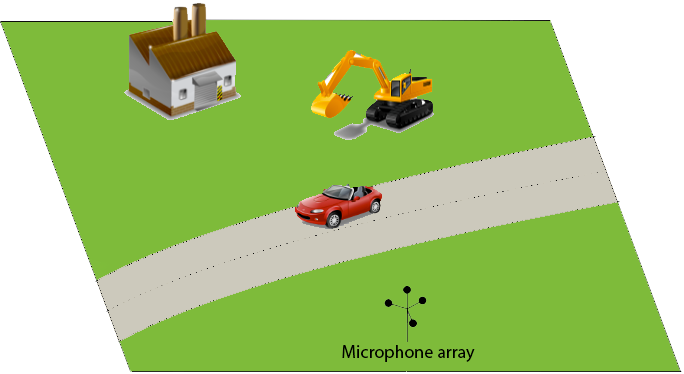
\includegraphics[width=0.8\textwidth]{Figures/scenariofarfield.png}
    \caption{Various outdoor sound sources being localized by a microphone array}
    \label{fig:Introductioncase}
\end{figure}

\section{Scope and outline of the thesis}

This thesis focus mainly on source signal spectrum ranging from low-to-mid frequencies in the far field. It should be noted that the purpose of this thesis is not to track moving sources, rather the thesis tackles the problem of \textit{static outdoor sound levels and their contributors} with the constraint of using as few microphones as possible while being robust to different noise and weather conditions. The thesis propose a solution capable of retrieving the noise source position in a variety of scenario including free-field to moderate reverberating environments. While previous research mostly tackle the problem of single source localization using linear or circular arrays, this thesis use a tetrahedral array to capture the signals.

The organization of the thesis is as follows: Chapter 2 derives the theory used to analyze the problem and create our simulation framework. Chapter 3 focus on describing the methods employed to solve the problem as well as algorithm features and its robustness and performance in outdoor conditions the algorithm performance.
Chapter 4 contains experimental results, anechoic and outdoor measurements investigating the algorithm limits in a variety of scenario.
Chapter 5 encompass a discussion about the solution and propose new ideas and further work.





\section{Direction of arrival using time delay information}
\subsection{Time delay between a single microphone pair}\label{sec:TDOA}

When using a pair of microphones, sound from a particular source arrives at the two microphones at different times, based on the source distance to the particular microphone. For a pair of microphones located at $m_{1}$ and $m_{2}$, the time difference of arrival (TDOA) of a sound signal from a source located at s can be defined as:
\begin{equation}
    \begin{split}
    T(\{m_{1},m_{2}\},s)&=\frac{|s-m_{1}|-|s-m_{2}|}{c}\\
                        &=\frac{|D_{1}|-|D_{2}|}{c}
    \label{eq:tdoa}
    \end{split}
\end{equation}
where c is the speed of sound in the medium and $|D_{1}|$ and $|D_{2}|$ the distance between the source and the microphones at $m_1$ and $m_2$.

In 2D, this equation leads to a hyperbola (Fig.\ref{eq:tdoa}) where the two focus points of the hyperbola are the sensors. The difference of the distance from any point of the hyperbola to the two focus is always the same.

\begin{figure}[H]
    \centering
    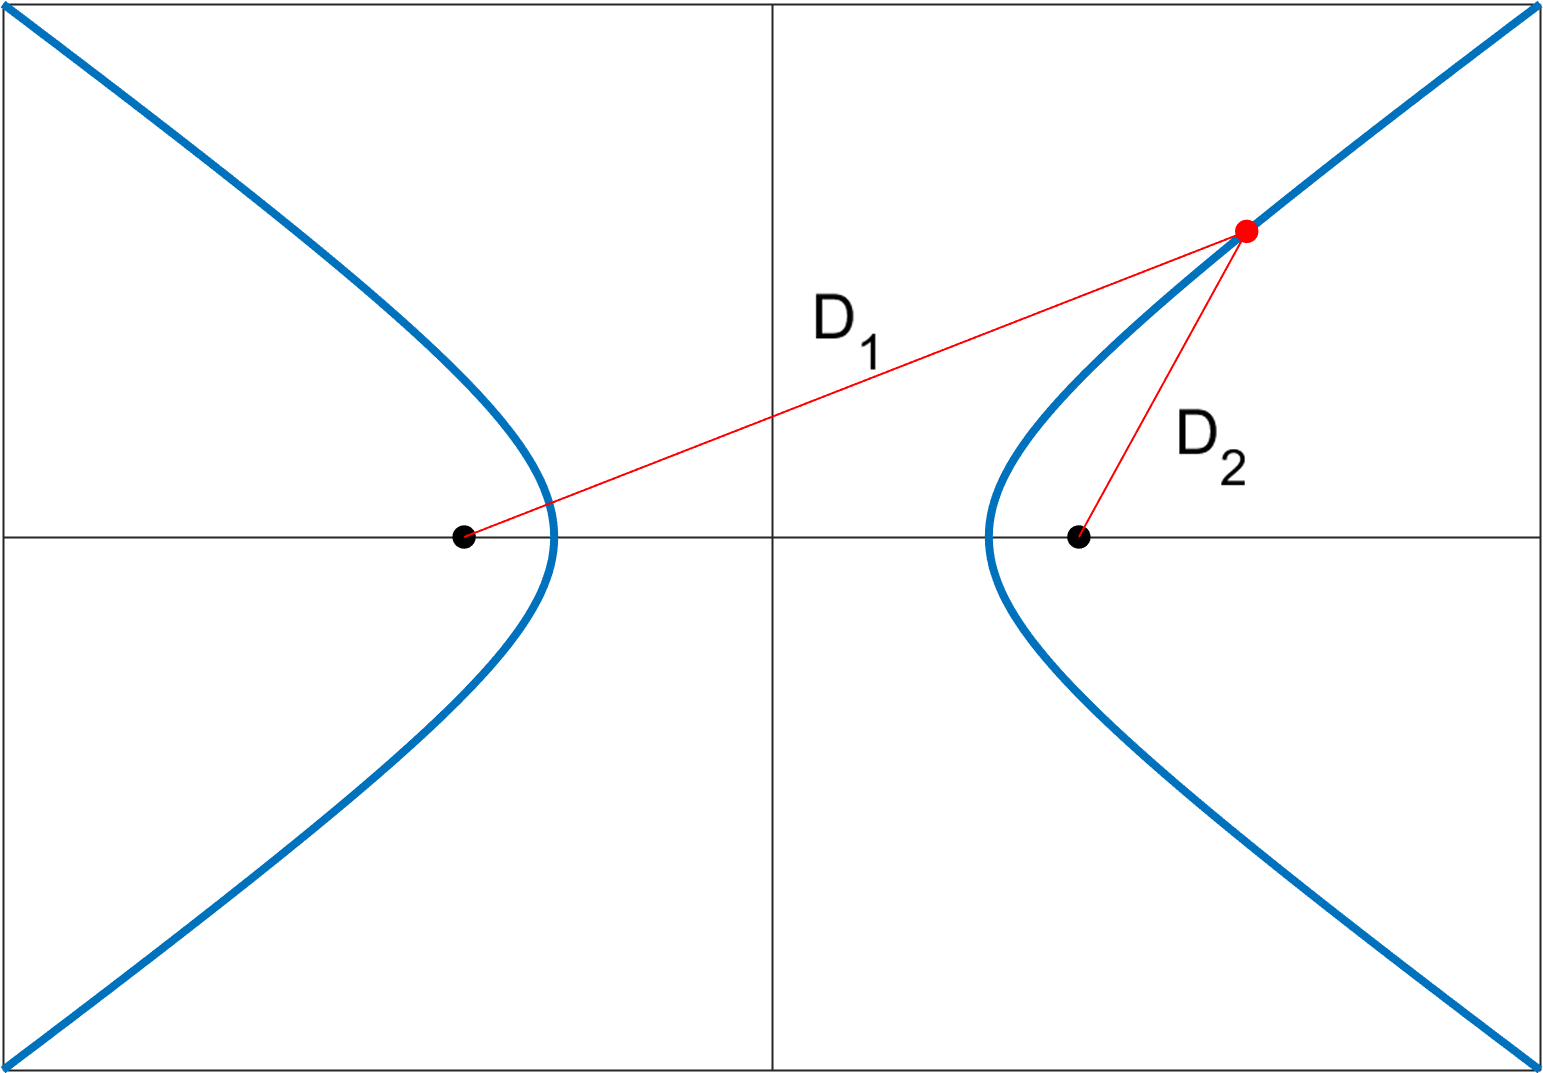
\includegraphics[width=0.8\textwidth]{Figures/hyperbola.png}
    \caption{A hyperbola (represented in blue), the red dot is any point on the hyperbola, the black dots represent the two foci. For any point on the hyperbola, $|D_1|-|D_2| = constant$}
    \label{eq:tdoa}
\end{figure}

In 3D, the TDOA information can be used to locate the source on a two-sheeted hyperboloid $\chi(\{m_{1},m_{2}\},s)$ such that the microphone positions are its foci. In practice the two-sheeted hyperboloid can be approximated to a cone so as to have a much simpler equation for the locus: $\theta$  = \textit{constant}, where $\theta$ is the angle of the source to the  midpoint of the line segment joining the two microphones (Fig. \ref{fig:hyperboloid_Cone}).

\begin{figure}[H]
    \centering
    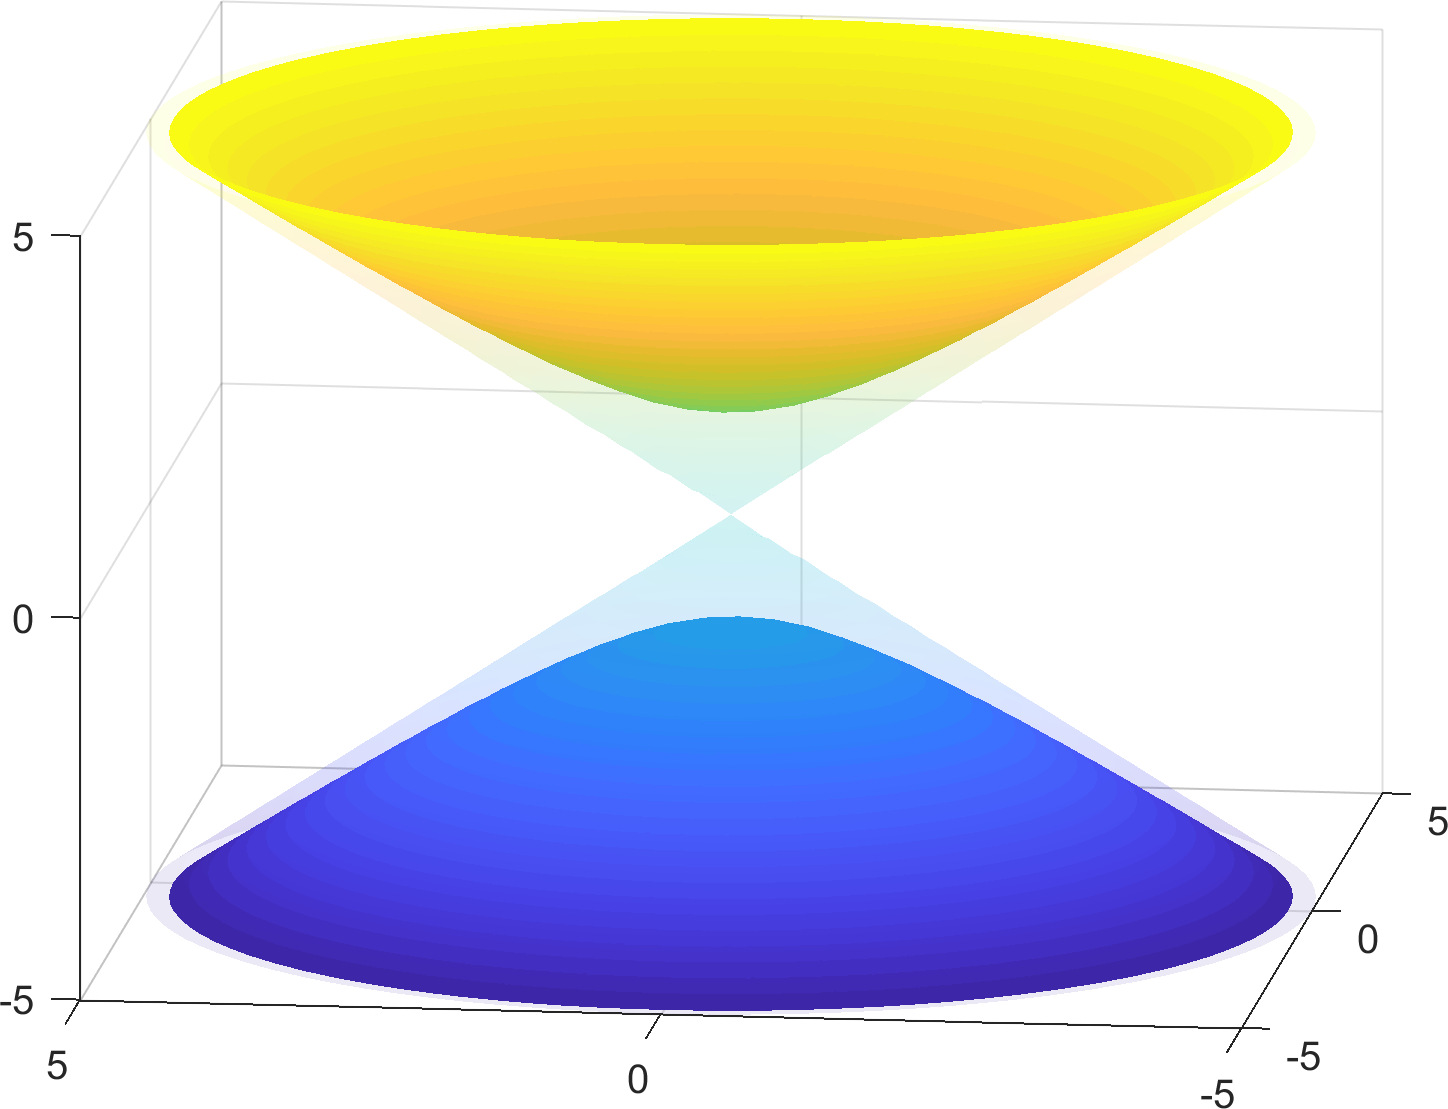
\includegraphics[width=0.8\textwidth]{Figures/hyperboloid.png}
    \caption{A 2-sheeted hyperboloid with a cone approximation overlay. As the tips of the hyperbola get closer (the microphones are closer), the hyperbola approximates the cone better.}
    \label{fig:hyperboloid_Cone}
\end{figure}

Of course as the source location gets closer to being orthogonal to the midpoint of the line segment joining the two microphones ($\theta=90\degree$), the hyperbola gets wider and flatter (more planar) and approximates the cone better. Also as the source gets closer to the line joining the two microphones ($\theta=0\degree, 180\degree$), the hyperbola collapses to a straight line and approximates the cone better. Thus, the error minimizes for broad-side sound source ($\theta=90\degree$) and for end-side sound source ($\theta=0\degree, 180\degree$), and maximizes for the midsection ($\theta=45\degree, 135\degree$). The equation for the error is given by
\begin{equation}
\begin{split}
    max\{\theta_{error}\} \approx  \frac{M_{dist}^2}{16R^2}\\
    max\{D_{error}\} \approx  \frac{M_{dist}^2}{16R},
\end{split}
\end{equation}
where $D_{error}$ is the actual source distance error (the gap between the cone and the hyperboloid) \cite{Brandstein:1995:FSS:922154}.

Microphones in microphone arrays are usually closely spaced with respect to the actual source distance, so the cone approximation works well. In most scenarios errors due to noise from other system parameters are greater than the errors associated with this approximation. Thus, given the time delay information between a microphone pair, the source can be located at a particular direction $\theta$, associated with the cone for that time delay. 

It can be shown that the cone approximation is the same as a far-field assumption for the sound source. The far-field assumption leads to a planar wave-front for a uniform linear microphone array. Thus, for the far-field, the DOA estimation problem is essentially the same as the TDOA estimation problem.

[FIG FOR FAR FIELD HERE !!!]

Now, given the TDOA between multiple microphone pairs, the source localization problem can be solved by triangulation. This triangulation problem can be solved for different variables ($\theta$, Source Distance or the Time Delay itself). The next section will detail the basics of solving such a problem. 

\subsection{TDOA of N pair of microphones}\label{sec:TDOAN}

Each pair i of sensor gives a locus $\chi{i}(\{m_{i1},m_{i2}\},s)$ on which the source can be located. When more than one pair of sensor is used, the position of the source can be found at the intersection of each locus. Depending on the position of each sensor pair and the direction of arrival of the source, the intersection of all the locus could in theory be found $ ( s\in {\bigcap}_{i=0}^k \chi{i} )$. In practical, the DOA is corrupted by random noise process which influence the localization precision and therefore the locus of each microphone pair. In most case, the locus intersection is the empty set. $ ( {\bigcap}_{i=0}^k \chi{i} = \emptyset ) $


Figure \ref{fig:hyperboloid_intersect} gives a 2D representation of 3 hyperboloid intersecting. The problem is therefore how to estimate the best intersection and how does this estimation influence our TDOA. Solution to this problem are discussed in section \ref{sec:LSTDOA}

\begin{figure}[H]
    \centering
    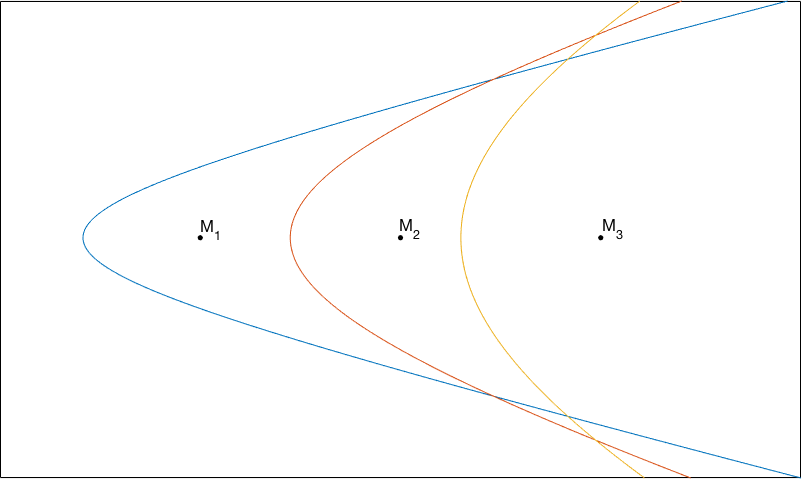
\includegraphics[width=0.8\textwidth]{Figures/intersect.png}
    \caption{2D representation of 3 locus. As seen above the intersection of the 3 locus is the empty set. $M_{1}$ , $M_{2}$ and $M_{3}$ represent the sensor position}
    \label{fig:hyperboloid_intersect}
\end{figure}

\subsection{Least Square problem}\label{sec:LSTDOA}

Let's define a Least Square (LS) problem which solves the localization of the sources in space as explained in section \ref{sec:TDOAN}. The LS problem optimize the position of the source in space by minimizing a given error criterion $ J $.
\begin{equation}
\hat{s}= \argmin_{s} J(s) 
\end{equation}

Traditionally, the literature define 3 errors criterion for solving the source location LS problem:  $J_{TDOA}(s)$, $J_{DOA}(s)$, $J_{D}(s)$. Those criterion are explains in the following sections.

\subsubsection{$J_{TDOA}(s)$ Error Criterion}

$J_{TDOA}(s)$ is the squared error difference between the time delay estimate $\tau$ and the time delay measured between the microphone pairs. The criterion and the optimization problem is given in the following.

\begin{equation}
J_{TDOA}(s) = {\sum}_{i=0}^k \epsilon_{itdoa}.[\tau_{i}-T(\{m_{i1},m_{i2}\},s)]^2
\label{eq:jtdoa}
\end{equation}
\begin{equation}
\hat{s}_{tdoa}= \argmin_{s} J_{tdoa}(s) 
\end{equation}

Assuming that the TDOA estimates $\tau_{i}$ are independently corrupted by zero-mean white gaussian noise, the stochastic variable $\mathcal{T}_{i}$ associated with this random process follows a normal distribution. The likelihood function of such a distribution is well-known and therefore the log of the distribution likelihood can be maximized yielding the Maximum Likelihood (ML) estimate of the TDOA from which the estimated position can be computed . 

Note that the error criterion is scaled by a factor $\epsilon_{itdoa}$ which is the inverse of the TDOA estimate $\mathcal{T}_{i}$ variance. 

\begin{equation}
\epsilon_{itdoa}=\frac{1}{\mathrm{Var}{\mathcal{T}_{i}}}
\label{eq:epsilonjtdoa}
\end{equation}

\subsubsection{$J_{DOA}(s)$ Error Criterion}

This is a classical formulation of the problem, which follows the same idea as the TDOA error criterion but this time the $J_{DOA}(s)$ is the squared error difference between the DOA estimate $\theta$ and the DOA measured between the microphone pairs. 

\begin{equation}
J_{DOA}(s) = {\sum}_{i=0}^k \epsilon_{idoa}.[\Theta_{i}-\theta(\{m_{i1},m_{i2}\},s)]^2
\label{eq:jdoa}
\end{equation}
\begin{equation}
\hat{s}_{doa}= \argmin_{s} J_{doa}(s) 
\end{equation}


Assuming that the DOA estimates $\theta_{i}$ are independently corrupted by zero-mean additive white Gaussian noise, the stochastic variable $\Theta_{i}$ associated with this random process follow a normal distribution. The error criterion is also scaled by a factor $\epsilon_{idoa}$ which is the inverse of the DOA estimate $\Theta_{i}$ variance. 

\begin{equation}
\epsilon_{idoa}=\frac{1}{\mathrm{Var}{\Theta_{i}}}
\label{eq:epsilonjtdoa}
\end{equation}

\subsubsection{$J_{D}(s)$ Error Criterion}

finally, $J_{D}(s)$ is the squared error difference between the orthogonal distance from s to the appropriate cone approximation 

\begin{equation}
J_{DOA}(s) = {\sum}_{i=0}^k \epsilon_{id}.[D(\chi_{i},s)]^2
\label{eq:jd}
\end{equation}
\begin{equation}
\hat{s}_{d}= \argmin_{s} J_{d}(s) 
\end{equation}


\begin{equation}
D(\chi_{i},s)=R_{i}.\sin{[\theta_{i}-\Theta(m_{i1},m_{i2},s)}]  
\end{equation}

\begin{equation}
 \epsilon_{id}=\frac{1}{\mathrm{Var}{\Theta_{i}}}    
\end{equation}

\subsubsection{Estimator performance}

The estimators described above vary in term of performance under certain conditions. For a bi-linear array, Brandstein has shown that $J_{TDOA}(s)$ and $J_{DOA}(s)$ are more robust to great angle of incidence than $J_{D}(s)$. At low noise level, $J_{TDOA}(s)$ is proven to be slightly better than $J_{DOA}(s)$ but $J_{DOA}(s)$ perform better overall especially for long range source location. $J_{TDOA}(s)$ is better for broadside sources and low noise level but $J_{DOA}(s)$ is more robust for less favorable noise conditions

%Pros and Cons of each estimators are sumarized in the following table.
\newpage
\section{Outdoor sound field modelling}
Various different models have been designed for outdoor sound field received at a receiver. The ISO 9613-2 \cite{ISO9613} is an international standard model for attenuation of sound when propagating outdoors. The standard uses an empirical method to quantify attenuation in different circumstances. This is a disadvantage as the model might not fit particular real world scenarios and user discretion is needed when using the model. NMPB-2008 \cite{dutilleux2010nmpb} is a French standard model which uses simple engineering methods to model road traffic noise. Over time it has been extended to include other sound sources. Nord2000 \cite{plovsing2000nord2000} and Harmonoise \cite{defrance2007outdoor} are more advanced engineering models for outdoor sound propagation. Nord2000 was developed in the period 1996-2001 by DELTA (Denmark, project manager, SINTEF (Norway), and SP (Sweden). Harmonoise is a more recent method and is made with a collaboration of various European countries. Nord2000 and Harmonoise are based on a similar approach and often produce quite similar models. Various inconclusive studies have been conducted comparing the two \cite{garg2014critical},\cite{jonsson2008comparison}. Eventually, to have a harmonized and coherent approach, a common framework for noise assessment (CNOSSOS-EU) was developed by the European Commission \cite{kephalopoulos2012common} in co-operation with the EU Member States to be applied for strategic noise mapping as required by the Environment Noise Directive (2002/49/EC). CNOSSUS-EU investigates the various existing methods and their advantages and disadvantages. It takes into consideration the accuracy as well as the computational complexities of the various methods. In general, the effect of different factors on outdoor sound propagation are described below.
\subsection{Spreading loss} 
The sound intensity from an omni-directional sound source drops as a function of distance due to wavefront spreading. The intensity I received at distance r from a source with power P, is given by
\begin{equation}
    I = \frac{P}{4\pi r^2}.
\end{equation}
This is due to spherical propagation, where the surface of the sphere has area $4\pi r^2$. In logarithm form this becomes
\begin{equation}
\begin{split}
    10log(I) &= 10log(\frac{P}{4\pi r^2}) \\
    L_p &= L_w - 20 log(r) - 11,
\end{split}
\end{equation}
which means a reduction of $20log2 = 6 dB$, every doubling of r. This equation assumes uniform omni-directional directivity. For directional sources a Directivity Index DI can be added giving
\begin{equation}
    L_p = L_w + DI - 20 log(r) - 11.
\end{equation}
It is important to remember that such a directivity can be inherent to the source or might be induced due to the location of the source. An omni-directional source placed on a perfectly reflecting plane can only propagate sound into a hemisphere, in which case the DI is 3 dB.  
An infinite line source can be viewed as a linear array of omni-directional point sources. The wavefront spread is cylindrical (surface area $= 2\pi r$),  which gives
\begin{equation}
\begin{split}
    10log(I) &= 10log(\frac{P}{2\pi r}) \\
    L_p &= L_w - 10 log(r) - 8,
\end{split}
\end{equation}
The DI is again 3 dB and the reduction is $10log2 = 3$ dB, every doubling of r. Highway traffic is modelled in a similar manner, assuming 3 dB drop every doubling of distance.
\subsection{Ground effects}
On acoustically hard surfaces such as non-porous asphalt or concrete, ground effects cause sound pressure to approximately double across a wide range of frequency. For porous surfaces, lower frequencies are enhanced while the higher frequencies get absorbed by the ground. When both source and receiver are close to the ground, interference of sound travelling directly from  source-to-receiver and sound reflected from the ground causes various ground effects. This interference can be both constructive or destructive. The pressure at a location $(x,y,z)$ due to a sound source can be given as a sum of the direct wave component, $P_{dir}$ and the reflected wave component $P_{ref}$ multiplied with the reflection coefficient R,
\begin{equation}
    P(x,y,z)=P_{dir}(x,y,z)+R.P_{ref}(x,y,z),    
\end{equation}
Here, $P_{dir} \neq P_{ref}$ as the two might have different propagation path lengths $r_ {dir}$ and $r_{ref}$. We have,
\begin{equation}
    P(x,y,z)=\frac{e^{-ikr_{dir}}}{4\pi r_{dir}} + R.\frac{e^{-ikr_{ref}}}{4\pi r_{ref}},
\end{equation}
For plane waves, the reflection coefficient of sound waves reflecting from the ground at angle $\phi$ is given by
\begin{equation}
    R = \frac{cos (\phi) - \beta}{cos (\phi) + \beta},
\end{equation}
here $\beta$ is specific normalized admittance of ground with respect to air. For infinitely hard surfaces $\beta \to 0$ and $R \to 1$. For infinitely soft surfaces  $\beta \to \infty$ and $R \to -1$. This can be interpreted as a phase change upon reflection from acoustically soft surfaces, which causes destructive interference and can also be seen as ground absorption. Note that for large distances, $\phi \to 90\degree$ (grazing incidence),  $r_2 \to r_1$ which makes $P_{ref} \to P_{dir}$ causing
\begin{equation}
\begin{split}
    P_{plane}(x,y,z)&=P_{dir}(x,y,z)+ \frac{0-\beta}{0+\beta}.P_{dir}(x,y,z)\\
            &=0.
\end{split}
\end{equation}
This predicts a net zero field over large distances irrespective of the value of $\beta$. The plane wavefront assumption is the cause of this error. Taking spherical waves, the equation for pressure becomes (Chap. 2 \cite{attenborough2006predicting})
\begin{equation}
    P(x,y,z)=\frac{e^{-ikr_{dir}}}{4\pi r_{dir}} + [R + (1-R)F(\omega)]\frac{e^{-ikr_{ref}}}{4\pi r_{ref}}
    \label{Eq:SphPressure}
\end{equation}
The $F(\omega)$, known as the boundary loss factor, is given by
\begin{equation}
    F(\omega)=1-i\sqrt{\pi}\omega e^{-\omega^2}\text{erfc}(i\omega).
\end{equation}
The $\omega$, often called the numerical distance, given by
\begin{equation}
    \omega \approx \frac{1}{2}(1+i)\sqrt{kr_{ref}}(cos(\phi)+\beta)
\end{equation}
and finally the erfc(i$\omega$) is known as the complementary error function given by 
\begin{equation}
    \text{erfc}(i\omega) = 1-\text{erf}(i\omega)
\end{equation}
where
\begin{equation}
    \text{erf}(i\omega)=\frac{1}{\sqrt\pi}\int_{-i\omega}^{i\omega}e^{-t^2}dt,
\end{equation}
which is a sigmoid shaped error function. Now by setting
\begin{equation}
    P_{plane}(x,y,z)=\frac{e^{-ikr_{dir}}}{4\pi r_{dir}} + R.\frac{e^{-ikr_{ref}}}{4\pi r_{ref}},
\end{equation}
and 
\begin{equation}
    P_{sph}(x,y,z)=(1-R)F(\omega).\frac{e^{-ikr_{ref}}}{4\pi r_{ref}},
\end{equation}
Eq. \ref{Eq:SphPressure} becomes
\begin{equation}
    P(x,y,z)=P_{plane}(x,y,z) + P_{sph}(x,y,z),
\end{equation}
here the $P_{sph}(x,y,z)$ contribution is known as the ground wave component. It corresponds to the contribution from the vicinity of the image source in the ground plane. It includes a component known as the surface wave, which propagates close and parallel to a porous ground surface and decays with inverse square root of range.
The ground itself impedes sound propagation by a variety of factors. Attenborough \cite{attenborough2011outdoor} created a more detailed 4-parameter model that requires porosity, flow resistivity, tortuosity and pore shape factor for modelling ground impedance on outdoor sound propagation. 
\subsection{Meteorological effects}
Wind and temperature have different effects on sound propagation. They directly change the speed of sound
\begin{equation}
    c_z = c_0\sqrt\frac{T+273.15}{273.15} + u_z,
\end{equation}
where $c_z$ is the speed of sound for temperature T above 0\degree C, $c_0$ is the speed of sound for no wind and 0\degree C, and $u_z$ is the wind velocity in the direction of propagation of sound. 

They also cause acoustic gradients (varying refractive index) to occur in the atmosphere. Usually, with increasing height, the temperature decreases. This causes sound to travel slower with height. In the absence of wind this causes the sound to refract upwards leading to less sound received at the receiver. Wind speed can increase or decrease the sound speed. Generally, speed of wind increases with height, which causes the sound travelling along the wind to refract downwards. Conversely, if the sound is travelling against the wind, this would cause the sound to refract upwards.
\begin{figure}[h]
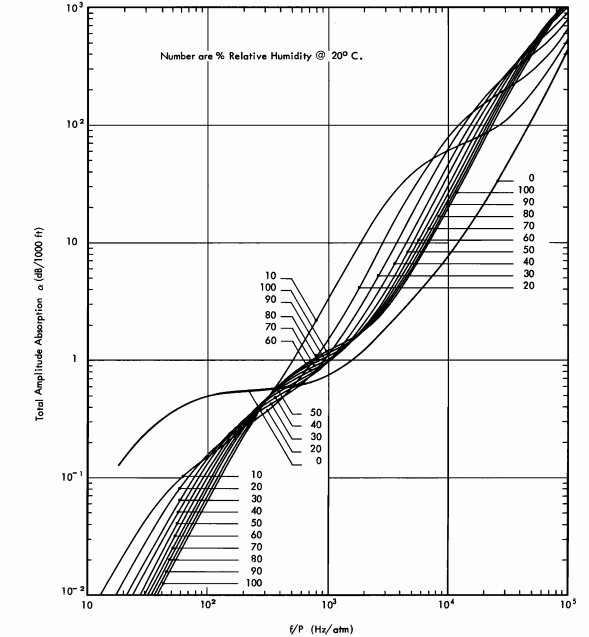
\includegraphics[width=0.8\textwidth]{Figures/airAbsorption.png}
\caption{Total absorption of sound in air as a function of frequency. The curves range from 0 to 100\% relative humidity and are for 20\degree C \cite{evans1972atmospheric} (Notice that the y-axis units are per 1000ft).}
\label{Fig:airAbsorption}
\end{figure}
\subsection{Atmospheric absorption}
Sound energy converts to heat as it travels through air. The conversion of sound-to-heat in air can happen due to conduction, shear viscosity or by molecular relaxation. The portion of sound absorbed by air becomes increasingly important as distance of propagation increases. For a plane wave, the loudness $L$ at a distance $x$ from a position of known loudness $L_0$ is given by
\begin{equation}
    L= L_0 - k.x,
\end{equation}
where k depends on the humidity, temperature, pressure as well as the molecular composition of atmosphere and is proportional to the square of the frequency. Thus, higher frequencies are absorbed by a far greater magnitude. This causes air to act as a low-pass filter over large distances. Molecular relaxation \cite{bass1990atmospheric}, \cite{evans1972atmospheric} is an important factor and losses due to oxygen-water vapour molecular relaxation are predominant above 500Hz. The absorption due to this factor is atleast 2 dB/kilometer irrespective of humidity and increases rapidly with frequency. The total absorption below 200 Hz is less than 1 dB/kilometer and decreases with frequency. If the air is extremely dry ($< 10\%$ relative humidity), the oxygen-carbon dioxide relaxation becomes significant and causes an almost constant absorption down from 500Hz to 80Hz of around 2dB/kilometer. The total air absorption as a function of frequency can be seen in Fig. \ref{Fig:airAbsorption}.
\subsection{Diffraction and barriers}
Barriers are sometimes purposefully built to block the direct path from the sound source to the receiver. Sound reaches the receiver either going through the barrier or by diffracting around the top of the barrier. Ground reflections and multi-path-propagation may lead to multiple diffracted wave paths. For a barrier, the ISO 9613-2 \cite{ISO9613} provides the following equation for loss due to barrier insertion
\begin{equation}
    IL = 10log\bigg[3+\bigg(C_2\frac{\delta_1}{\lambda}\bigg)C_3K_{met}\bigg],
\end{equation}
where $\lambda=wavelength$. The value of $C_2$ determines if ground reflections are taken care of ($C_2 = 20$) or not ($C_2 = 40$), $C_3$ is a factor to take care of double diffraction due to a barrier of finite thickness (or two thin barriers placed some distance apart), $\delta_1$ is the difference in distance between the direct source-to-receiver path and the wave propagation path caused by the barrier, and $K_{met}$ is a correction factor for average downwind meteorological effects. For thin barriers the equation simplifies to 
\begin{equation}
    IL = 10log(3+40\frac{\delta_1}{\lambda}). 
\end{equation}
Over large distances even buildings act like barriers, with the rooftop causing double diffraction. ISO 9613-2 \cite{ISO9613} provides a simple empirical method to calculate attenuation due to buildings.

\section{Acoustic Models}

Various methods have been used \cite{benesty2008microphone} to solve the estimation problem discussed in the previous section. The estimation problem would be trivial if the source signals received at each of the different microphones were simply delayed and scaled versions of each other. However, the source signal at each microphone is generally intermixed with surrounding noise. On top of that it contains attenuated and distorted copies of itself due to boundary reflections (if the measurement is not being made in free field or its approximation like an anechoic chamber). Add to this the fact that the source itself might be moving leading to a changing TDOA to the different microphones. All these factors quickly convert TDOA estimation to a non-trivial problem. \\
Based on these factors, the problem can be solved for assuming a variety of acoustical models. Beginning for a single source in a free-field (non-reverberant), to a single-source in a reverberant environment, to multiple-sources in a free-field or reverberant environments, and lastly, multiple-moving-sources. The following section will formulate each of these models.

\subsection{Formulation of possible acoustic models}
Suppose our sources are in a sound field with an array of N microphones. Then the different possible acoustic models for TDOA analysis can be formulated as below.

\subsubsection{Single-source in free-field}
Let the acoustic signal from the single-source be \textit{s(k)} at time k. Then the signal received by the $n^{th}$ microphone at time k can be given be divided into the signal $x_n(k)$ and noise $\eta_n(k)$
\begin{equation}
    \begin{split}
    y_n(k) &= x_n(k) + \eta_n(k),\hspace{10pt} n = 1,2,....,N\\ 
           &=\alpha_n s(k-t-\tau_{n1}) + \eta_n(k),
    \end{split}
\end{equation}
where $\alpha_n$ is the gain/ attenuation of the signal at microphone n, t is the delay to the first microphone that receives the signal and $\tau_{n1}$ is the relative time delay of receiving signal between the first and the $n^{th}$ microphone, $\eta_n(k)$ being the noise at the $n^{th}$ microphone at time k. $\tau_{n1}$ can be defined as, $\tau_{n1}=\zeta(\tau)$, where, $\tau$ is the time delay between a pre-determined pair of microphones (say, microphone 1 and 2). Given $\tau$ and knowing the array geometry, it is possible to determine possible solutions for the rest of the delays between microphone pairs. Of course, there might not be a unique solution given a single value of $\tau$. $\zeta(\tau)$ can then be defined as a function of $\tau$ which can linear or a higher order polynomial depending on the array geometry. The estimation problem is then that of determining the estimate $\hat{\tau}$ of the true time delay $\tau$, given a finite number of observations.

\subsubsection{Multiple-sources in free-field}

For multiple sources (m = 1,2,....M), the signal received at $n^{th}$ microphone can be defined as : 
\begin{equation}
    \begin{split}
         y_n(k) &= x_n(k) + \eta_n(k),\hspace{10pt} n = 1,2,....,N \\
                &= \sum\limits_{m=1}^M \alpha_{nm}s_m[k - t_m - \zeta({\tau_m})] + \eta_n(k),
    \end{split}
\end{equation}
which is similar to the equation for the single-source, except the gain factor and the signal now depend on the $m^{th}$ source, so the total signal received at $n^{th}$ microphone is the sum of the signals from all M sources. The estimation problem is then that of determining all the estimates $\hat{\tau}_m$ of the true time delays $\tau_m$, given a finite number of observations.

\subsubsection{Single-source in reverberant-field}

For a single source in a reverberant field, finding the delay is not a simple problem. A reverberant field can be represented by a sufficiently long FIR filter, which adds multiple delayed and attenuated version of the source signal to the received signal, the number depending on the number of taps on that filter. The signal received at the $n^{th}$ microphone can be given by
\begin{equation}
    \begin{split}
         y_n(k) &= x_n(k) + \eta_n(k),\hspace{10pt} n = 1,2,....,N \\
                &= g_n*s(k) + \eta_n(k),
    \end{split}
\end{equation}
where $g_n$ is the impulse response from the source to the $n^{th}$ microphone. 
The $g_n$ then signifies a filter which adds multiple attenuated copies of the source signal at the receiver due to reverberation and also the actual source signal delay. So, the true delay for the same source signal on different microphone is hidden in this filter. It can be thought of as a multiple source problem, but all the sources are playing the same signal. The problem then is of separating these multiple sources with the knowledge of the reverberant field. If the goal is room auralization then the reverberation needs to be captured as image sources, however if the goal is source localization, then a technique needs to be devised so that the reverberation effect is filtered converting the problem to an approximation of the single-source in a free field model. 

\subsubsection{Multiple-sources in reverberant-field}
More on this soon!!
%\section{Tetrahedral microphone array}
A unit vector $\overline{u}$ in 3d space can be defined in spherical coordinates by (1,$\theta$,$\phi$), where the magnitude of the vector is 1, $\theta$ the azimuth and $\phi$ the elevation [3d space point fig here]. We get
\begin{equation}
    \begin{split}
        x_u&=cos(\theta)cos(\phi) \\
        y_u&=sin(\theta)cos(\phi) \\
        z_u&=sin(\phi),
    \end{split}
\end{equation}
this can be denoted by the unit propagation vector ${a(\theta,\phi)}$ in the Cartesian coordinates
\begin{equation}
    a(\theta,\phi)=\begin{bmatrix}cos(\theta)cos(\phi) \\sin(\theta)cos(\phi) \\sin(\phi)\end{bmatrix},
\end{equation}
Suppose sound is travelling along the unit vector $\overline{u}$. Let 2 microphones be placed at positions $\overline{p_1}=(x_1,y_1,z_1)$ and $\overline{p_2}=(x_2,y_2,z_2)$.  Then $\overline{p_{12}}=\overline{p_{2}}-\overline{p_{1}}$, where ${\overline{p_{12}}}$ is the distance between the two microphones. The projection of this distance in the direction of $\overline{u}$ is simply $a(\theta,\phi)\overline{p_{12}}$ and the time it takes for sound to travel between the two microphones is then 
\begin{equation}
    T_{12}=\frac{a(\theta,\phi)\overline{p_{12}}}{c},
\end{equation} c being the speed of sound. For 4 microphones, a Least-Squares approach could be considered, with $^4C_2$ combinations possible. The 'correct' DOA is then the $a(\Theta,\Phi)$ which minimizes the cost function
\begin{equation}
    J(\Theta,\Phi) = \sum\bigg(T_{ij}-\frac{a(\Theta,\Phi)\overline{p_{ij}}}{c}\bigg)^2, \text{for } i,j \in \begin{pmatrix}4\\2\end{pmatrix}.
\end{equation}

Using atleast 4 microphones a spatial array can be constructed. The simplest spatial structure with 4 vertices is a tetrahedron (a triangular pyramid). The tetrahedron has 4 vertices, 4 faces and 6 edges. If the tetrahedron is regular then all the vertices are equally spaced from each other and every face is an equilateral triangle.The following section discusses the simulated performance of different TDOA and DOA algorithms on a tetrahedral array in an outdoor environment.

\subsection{Regular tetrahedral array}

%Let's define a regular tetrahedral array geometry as follows
%\begin{equation}
%    \begin{split}
%        p_1 &= \begin{bmatrix}{-0.5} & {0} & {0}\end{bmatrix}^T \\
%        p_2 &= \begin{bmatrix}{0.5} & {0} & {0}\end{bmatrix}^T \\
%        p_3 &= \begin{bmatrix}{0} & {\sqrt{(0.75)}} & {0}\end{bmatrix}^T \\
%        p_4 &= \begin{bmatrix}{0} & {\sqrt{(0.75)/2}} & {\sqrt{(0.5)}}\end{bmatrix}^T,
%    \end{split}
%\end{equation}


\begin{figure}[H]
    \centering
    \begin{subfigure}[b]{0.48\textwidth}
    \centering
    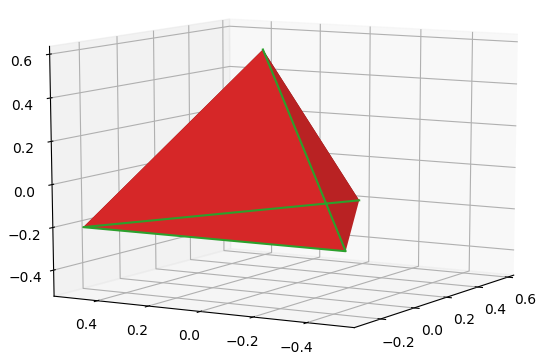
\includegraphics[width=0.9\textwidth]{Figures/unit_tetra.png}
    \caption{Frontal view}
    \label{fig:d1}
\end{subfigure}
\hfill
\begin{subfigure}[b]{0.48\textwidth}
    \centering
    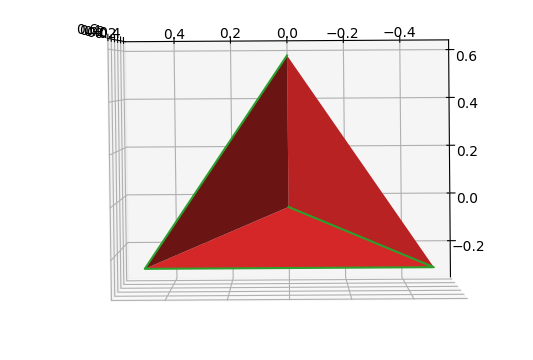
\includegraphics[width=0.9\textwidth]{Figures/unit_tetra_top.png}
    \caption{Top view}
    \label{fig:d2}
\end{subfigure}
    \caption{Representation of a regular Tetrahedral with unit side, centroid at origin and horizontally level lower face, front view and top view}
    \label{fig:regulartetra}
\end{figure}

The distance between the microphones (array aperture) for the tetrahedron in Fig. \ref{fig:regulartetra} is 1m. For such an array, spatial aliasing would occur for frequencies $> (c*1m)/2 \approx $170Hz, c being the speed on sound.  When Fourier based techniques are used for non-stationary signal, the spatial frequency must satisfy the Nyquist Frequency (i.e be $< c/2$) but this requirement can be relaxed for a stationary signal by using anti-aliasing techniques \cite{dmochowski2009spatial}. Fig. \ref{fig:directivityregulartetra} shows the directivity of a tetrahedral array for various frequencies. As expected, aliasing occurs and the main lobe disappears for frequencies $> c/2$. Fig. \ref{fig:directivityothers} shows the directivity for a 4-element uniform linear array (ULA) and uniform circular array (UCA) with the same array aperture of 1m. Since no elevation information can be retrieved from a uni-dimensional linear array the directivity pattern is donut shaped, meaning that the source is located somewhere on the donut. 


\begin{figure}[H]
\centering
\begin{subfigure}{.5\textwidth}
    \centering
        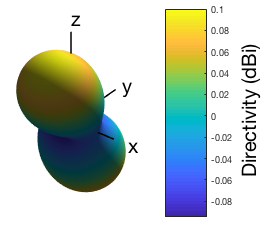
\includegraphics[width=0.7\textwidth]{Figures/regulartetra50hzdirectivity.png}
    \label{fig:directivity200hzregulartetra}
\end{subfigure}%
\begin{subfigure}{.5\textwidth}
        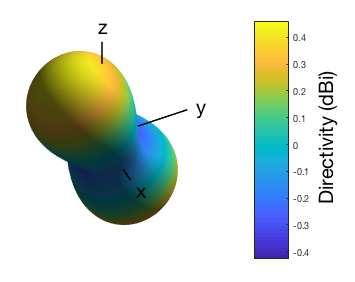
\includegraphics[width=0.7\textwidth]{Figures/regulartetra100hzdirectivity.png}
    \label{fig:directivity100hzregulartetra}
\end{subfigure}
\begin{subfigure}{.5\textwidth}
    \centering
        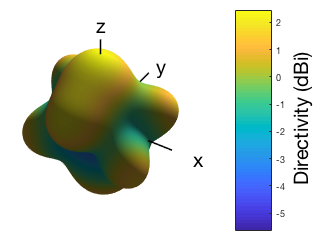
\includegraphics[width=0.9\textwidth]{Figures/regulartetra200hzdirectivity.png}
    \label{fig:directivity200hzregulartetra}
\end{subfigure}%
\begin{subfigure}{.5\textwidth}
    \centering
        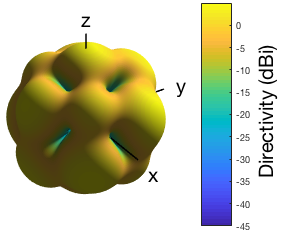
\includegraphics[width=0.9\textwidth]{Figures/regulartetra400hz.png}
    \label{fig:directivity400hzregulartetra}
\end{subfigure}
\caption{Directivity of the regular tetrahedral array at 50hz (top), 100hz(right), 200hz (bottom left) and 400hz (bottom right)}
\label{fig:directivityregulartetra}
\end{figure}


\begin{figure}[H]
\centering
\begin{subfigure}{.5\textwidth}
    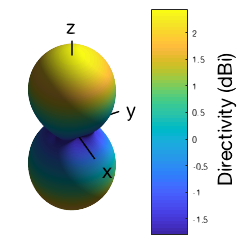
\includegraphics[width=0.85\textwidth]{Figures/uca100hzdirectivity4mic.png}
    \label{fig:directivity100hzuca}
\end{subfigure}%
\begin{subfigure}{.5\textwidth}
    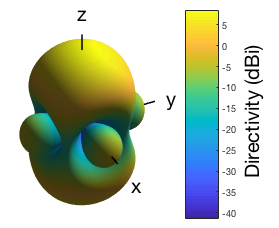
\includegraphics[width=0.85\textwidth]{Figures/uca200hzdirectivity4mic.png}
    \label{fig:directivity100hzuca}
\end{subfigure}%
\caption{Directivity of the UCA array at 100hz(left) and 200hz (right)}
%\label{fig:test}
\end{figure}

\begin{figure}[H]
\centering
\begin{subfigure}{.5\textwidth}
    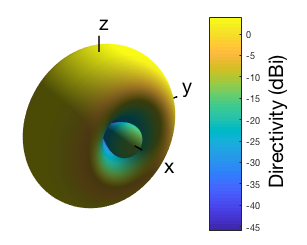
\includegraphics[width=0.85\textwidth]{Figures/ula100hzdirectivity.png}
    \label{fig:directivity100hzuca}
\end{subfigure}%
\begin{subfigure}{.5\textwidth}
    \centering
    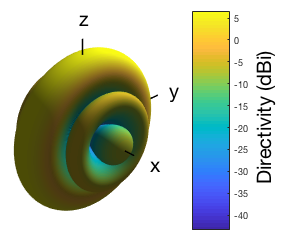
\includegraphics[width=1.1\textwidth]{Figures/ula200hzdirectivity.png}
    \label{fig:directivity100hzula}
\end{subfigure}
\caption{Directivity of the ULA array at 100hz (left) and 200hz (right)}
\label{fig:directivityothers}
\end{figure}
\section{Methods}
\subsection{Generalized correlation method}
The famous Knapp-Carter paper details the generalized cross-correlation method (GCC) for estimation of time delay \cite{1162830} in free field. For a pair of microphones, $m_1$ \& $m_2$, separated by a distance, the signals from a source received at time t can be given by
\begin{equation}
    \begin{split}
        x_1(t) &= s_1(t) + n_1(t) \\
        x_2(t) &= \alpha s_1(t - D) + n_2(t) ,
    \end{split}
\end{equation}
where $n_1(t)$ \& $n_2(t)$ are the noise at time t at the two microphones which are uncorrelated to the signal $s_1(t)$. The microphone $m_1$ receives the signal $s_1(t)$ first, while the microphone $m_2$ receives a delayed and attenuated version $\alpha s_1(t - D)$ at time t. The $\alpha$ depends on the microphone relative distance and microphone calibration and within-media factors like absorption. The time delay D depends on the microphone pair relative distance, the speed of sound in the media and the position of the sound source. 

Based on the discussions in previous sections, if we can estimate the value of D, we can estimate the source location. However, depending on source movement and environmental factors, both $\alpha$ and D can change over time. The estimation of D thus can only be made for observations of a finite duration. D can be estimated by computing the cross-correlation of the two signals
\begin{equation}
        R_{x_1x_2}(\tau) = \textbf{E[}x_1(t)x_2(t+\tau)\textbf], 
\end{equation}
Assuming noise to be uncorrelated to each other as well as the source signal, the cross correlation can be expressed as
\begin{equation}
    \begin{split}
        R_{x_1x_2}(\tau) &= \textbf{E[}\{s_1(t) + n_1(t)\}\{\alpha s_1(t+\tau - D) + n_2(t)\}\textbf] \\
                         &= \alpha\textbf{E[}s_1(t)s_1(t+\tau - D)\textbf] \\
                         &= \alpha R_{s_1s_1}(\tau - D),
    \end{split}
    \label{Eq:crosscorr}
\end{equation}
this cross-correlation peaks at $\tau - D = 0$, i.e. $\tau = D$. So the $\tau$ that maximizes the cross-correlation is an estimator for the time delay D. Assuming the processes to be ergodic so that the samples from a finite duration T can be used to estimate the cross-correlation, the estimate can be given by
\begin{equation}
    \hat{R}_{x_1 x_2}(\tau) = \frac{1}{T-\tau}\int_{0}^{T-\tau}x_1(t)x_2(t+\tau)dt,
\end{equation}
choosing sample mean as the estimator. Notice that even though the observation interval is T, we can only get usable information for time T - $\tau$, as we will have no corresponding signal for microphone $m_2$ for any signal that we receive at microphone $m_1$ after that time.

Taking the Fourier transform of Eq. \ref{Eq:crosscorr} to move to the frequency domain
\begin{equation}
        G_{x_1x_2}(f) = \alpha G_{s_1s_1}(f)\cdot e^{-j2\pi fD},
        \label{Eq:Gx1x2Gs1s1}
\end{equation}
multiplication with $e^{-j2\pi fD}$ in the frequency domain becomes convolution in the time domain
\begin{equation}
        R_{x_1x_2}(\tau) = \alpha R_{s_1s_1}(\tau) \circledast\delta(\tau - D),
        \label{Eq:Rx1x2}
\end{equation}
which can be seen as the Fourier transform of the signal spectrum spreading the delta function. The way to ensure no spreading takes place is to use a white noise signal. The autocorrelation of white noise is a delta function, in which case convolution with the delay-delta function results in a single peak value. Of course, in any kind of a reverberant field this will never be a single value. This is because the reverberations will have the effect of making the signal add up in a periodic and attenuated manner. However, the peak of the autocorrelation $R_{x_1x_2}(\tau)$ still happens at $\tau = D$, with the spreading having the effect of broadening the peak. If the time delay D is not a single value however, as can be the case in reverberant fields or for periodic signals, the $R_{x_1x_2}(\tau)$ will have multiple peaks. Each broad peak will overlap with the other in an additive or destructive manner making is impossible to detect or distinguish peaks. 

$R_{s_1s_1}(\tau)$ in Eq. \ref{Eq:Rx1x2} can be expanded to frequency domain to get
\begin{equation}
        R_{x_1x_2}(\tau) =  {\bigg[\int_{-\infty}^{\infty}\alpha{G}_{s_1s_1}(f) e^{-j2\pi f\tau} df\bigg]} \circledast\delta(\tau - D),
\end{equation}
this cross-correlation $R_{x_1x_2}(\tau)$ is a function that is spread around $\delta(\tau - D)$ according to ${G}_{s_1s_1}(f)$. This spreading is detrimental to the resolution of the localization results. Also, if the signal itself is non-stationary, like speech signals, this spreading is also unpredictable.

Now we are ready to form a basis for the different GCC weighing methods. If \textit{a priori} signal or noise information is available, the signals  $x_1(t)$ \& $x_2(t)$ can be pre-filtered to improve the accuracy of estimating the time delay. The method of selection of the pre-filter weights then forms the basis for the different GCC methods. 

Suppose, $x_1(t)$ \& $x_2(t)$ are filtered through filters $H_1(f)$ and $H_2(f)$, to get filtered signals $y_1(t)$ \& $y_2(t)$ respectively, then we have
\begin{equation}
        G_{y_1y_2}(f) = H_1(f)H^*_2(f) G_{x_1x_2}(f),
\end{equation}
taking the Fourier transform
\begin{equation}
\begin{split}
            R_{y_1y_2}(\tau) &= \int_{-\infty}^{\infty}H_1(f)H^*_2(f) G_{x_1x_2}(f) e^{-j2\pi f\tau} df \\
                             &= \int_{-\infty}^{\infty}\psi(f) G_{x_1x_2}(f) e^{-j2\pi f\tau} df,
\end{split}
\end{equation}
where 
\begin{equation}
            \psi(f) = H_1(f)H^*_2(f),
\end{equation}
since we can only estimate the cross-power spectra, we can write
\begin{equation}
            \hat{R}_{y_1y_2}(\tau) = \int_{-\infty}^{\infty}\psi(f) \hat{G}_{x_1x_2}(f) e^{-j2\pi f\tau} df,
\end{equation}
the frequency weights given by $\psi(f)$ can be selected according to the purpose that is wished to be achieved. For example, if the purpose is to maximize the signal-to-noise (SNR) ratio in the signal passed, then the $\psi(f)$ could be selected so that it attenuates the frequencies in the noise spectra. Obviously this requires either priori-knowledge or estimation of the noise spectra. The following sections introduce the different methods of frequency weight selection. Four methods are described here, ROTH, SCOT, PHAT and ML. Of particular interest are the PHAT and ML, direct and improved versions of which have been consistently used to do robust source localization. 

\subsubsection{ROTH}
The frequency weights for ROTH processor are defined as
\begin{equation}
            \psi(f) = \frac{1}{G_{x_1x_1}(f)},
\end{equation}
so we get 
\begin{equation}
            {R}_{y_1y_2}(\tau) = \int_{-\infty}^{\infty}\frac{{G}_{x_1x_2}(f)}{G_{x_1x_1}(f)} e^{j2\pi f\tau} df,
\end{equation}
substituting the value for ${G}_{x_1x_2}(f)$ assuming uncorrelated noise from Eq. \ref{Eq:Gx1x2Gs1s1} we get
\begin{equation}
\begin{split}
                \hat{R}_{y_1y_2}(\tau) &= \int_{-\infty}^{\infty}\frac{\alpha\hat{G}_{s_1s_1}(f)}{G_{x_1x_1}(f)} e^{j2\pi f.(\tau-D)} df \\
                                        &= \delta (\tau - D) \circledast \bigg[\int_{-\infty}^{\infty}\frac{\alpha\hat{G}_{s_1s_1}(f)}{G_{s_1s_1}(f) + G_{n_1n_1}(f)} e^{j2\pi f\tau}  df\bigg],
                                        %&= \delta (\tau - D) \circledast \alpha\bigg[\int_{-\infty}^{\infty}\frac{{G}_{s_1s_1}(f) + G_{n_1n_1}(f) -G_{n_1n_1}(f)}{G_{s_1s_1}(f) + G_{n_1n_1}(f)} e^{j2\pi f\tau}  df\bigg] \\
                                        %&= \delta (\tau - D) \circledast \alpha\bigg[\int_{-\infty}^{\infty}e^{j2\pi f\tau}df-\int_{-\infty}^{\infty}\frac{G_{n_1n_1}(f)}{G_{s_1s_1}(f) + G_{n_1n_1}(f)} e^{j2\pi f\tau}  df\bigg] \\
\end{split}
\end{equation}
so now the delta function is spread according to the value of $G_{n_1n_1}(f)$. For frequencies f where $G_{n_1n_1}(f)$ has a high magnitude, the cross-correlation will be suppressed, so that peaks in the frequency regions where $n_1$ is high disappear. But as can be seen ROTH processor does nothing to improve the high $n_2$ regions or the spreading around the main peak.

\subsubsection{SCOT}
The frequency weights for SCOT processor are defined as
\begin{equation}
            \psi(f) = \frac{1}{\sqrt{G_{x_1x_1}(f)G_{x_2x_2}(f)}},
\end{equation}
so this takes care of regions where either $n_1$ or $n_2$ might be high solving a possible disadvantage with ROTH. 

\subsubsection{PHAT}
Both SCOT and ROTH suffer from the disadvantage that the value of ${R}_{y_1y_2}(\tau)$ is spread around the delta function depending on the cross-spectrum ${G}_{x_1x_2}(f)$. However, the TDOA information is carried only by the phase of the cross-spectrum and not the amplitude. So, setting the weights as
\begin{equation}
            \psi(f) = \frac{1}{|G_{x_1x_2}(f)|},
\end{equation}
we get
\begin{equation}
        {R}_{y_1y_2}(\tau) = \int_{-\infty}^{\infty}\frac{{G}_{x_1x_2}(f)}{|G_{x_1x_2}(f)|}e^{j2\pi f\tau}   df,
\end{equation}
Now, we have from Eq. \ref{Eq:Gx1x2Gs1s1}
\begin{equation}
\begin{split}
        |G_{x_1x_2}(f)| &= \alpha G_{s_1s_1}(f) \\
    \frac{{G}_{x_1x_2}(f)}{|G_{x_1x_2}(f)|}&=e^{-j2\pi fD},
\end{split}
\label{Eq:ModGx1x2}
\end{equation}
where the magnitude information is cancelled and only the phase information remains, where D is the delay or the 'phase'. We get
\begin{equation}
\begin{split}
            {R}_{y_1y_2}(\tau) &= \int_{-\infty}^{\infty}e^{j2\pi f(\tau - D)}   df \\
                           &=  \delta (\tau - D) \circledast \int_{-\infty}^{\infty}e^{j2\pi f\tau} df,
\end{split}
\label{Eq:RY1Y2}
\end{equation}
So ideally PHAT weighing gives a cross-correlation value that has no spreading and gives a clean peak at $\tau=D$.

Even though PHAT seems to solve all problems, the method is not without issues. Most of the issues arise from the assumptions made for PHAT. These are itemized below: 
\begin{itemize}
    \item $n_1$ and $n_2$ are assumed to be uncorrelated. If that is not the case, the magnitude of $G_{x_1x_2}(f)$ would obviously not cancel out in Eq. \ref{Eq:ModGx1x2}
    \item The GCC methods assume single-source in free-field model, ie, no reverberation is assumed. The effects of reverberation can actually be moderate to severe in PHAT and have been discussed in various papers [Cite papers here]. 
    \item The 'expected' value of $G_{x_1x_2}(f)$ is assumed to be known. In reality it can only be estimated, viz $\hat{G}_{x_1x_2}(f)$. In situations where $\hat{G}_{x_1x_2}(f) \neq G_{x_1x_2}(f)$, the cross-correlation in Eq. \ref{Eq:RY1Y2} will not be a delta function. This error is magnified even more in regions where $G_{s_1s_1}(f)$ is very low. This has the potential to cause PHAT to provide poor results in low SNR conditions.
\end{itemize}  

A practical issue that exists with GCC methods is the angular resolution of localization. If the signals are recorded at 44.1kHz sample rate, then the minimum time delay allowed is $1/$ 44100 sec for 1 sample delay. For 2 microphones placed distance $20$ cm apart, the minimum resolution achievable in this time is $2.2\degree$ broadside to $16\degree$ endside, assuming speed of sound to be 343 m/sec (Fig. \ref{fig:ang_res}). At 192kHz and 1m microphone distance, the issue is less severe, being $0.5\degree$ broadside to $7.7\degree$ endside.
\begin{figure}[H]
     \centering
     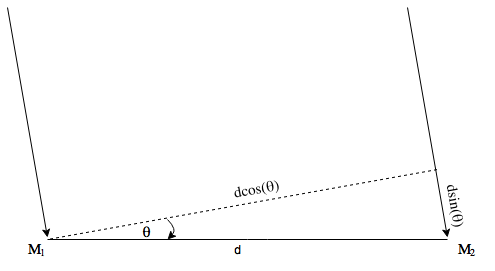
\includegraphics[width=0.8\textwidth]{Figures/AngularRes.png}
     \caption{Figure represents plane wave incidence on a microphone pair. For broadside incidence the time delay is the minimum = 0 between the two microphones. The next time delay allowed is $1/$fs, corresponding to travel distance of $c/$fs (c being the speed of sound). So we have  dsin($\theta$) = $c$/fs. For endside incidence the time delay is maximum = $d/c$. The next time delay allowed is $d/c$-$1/$fs, corresponding to travel distance of $d$-$c/$fs, and we have dsin($\theta$) =  $d$-$c/$fs.}
     \label{fig:ang_res}
\end{figure}

The issue is solved by curve fitting and interpolation. Parabolic curve fitting was initially proposed method to solve it, but was shown to be a biased estimator \cite{boucher1981analysis}. Consequently, various interpolation techniques have been developed to overcome this issue \cite{jacovitti1993discrete}, \cite{brandstein1997practical}, \cite{zhang2005cross}, \cite{tervo2008interpolation}. The 2D localization resolution with no interpolation is plotted in Fig. \ref{fig:res_diff}.

\begin{figure}[H]
    \centering
    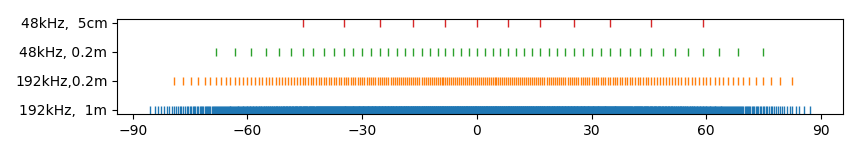
\includegraphics[width=\textwidth]{Figures/res_diff.png}
    \caption{Frontal 2D localization resolution for different sample rates and distance between a pair of microphones. As can be seen large apertures and high sample rates have a better resolution than lower sample rates and smaller apertures.}
    \label{fig:res_diff}
\end{figure}

Some simulations for GCC are given in Fig. \ref{fig:GCC_SIM}. It can be seen that the resolution falls the closer we get to end-side ($0\degree$ and $180\degree$). Also it can be seen that the results are poor if no weights are used. PHAT and SCOT perform quite similarly in the simulations, with PHAT being marginally better. It can be seen that the level difference is maintained between the 2 sources in the results. However no peaks are visible if the SNR falls to 0 dB.

\begin{figure}[H]
    \centering
    \begin{subfigure}[b]{0.48\textwidth}
    \centering
    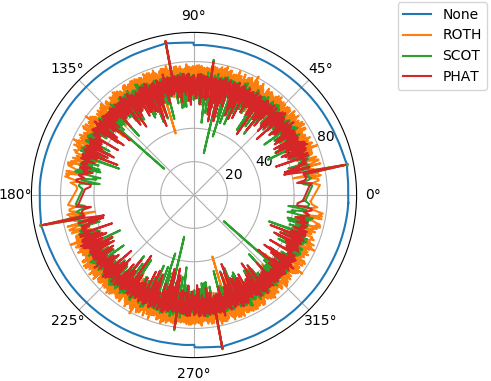
\includegraphics[width=0.9\textwidth]{Figures/GCC_40.png}
    \caption{Both sources at 40dB SNR}
    \label{fig:d1}
\end{subfigure}
\hfill
\begin{subfigure}[b]{0.48\textwidth}
    \centering
    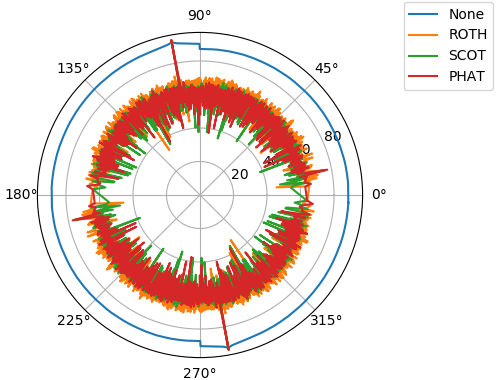
\includegraphics[width=0.9\textwidth]{Figures/GCC_20_40.png}
    \caption{S1 at 20dB SNR, S2 at 40dB SNR}
    \label{fig:d2}
\end{subfigure}
\vskip \baselineskip
\begin{subfigure}[b]{0.48\textwidth}
    \centering
    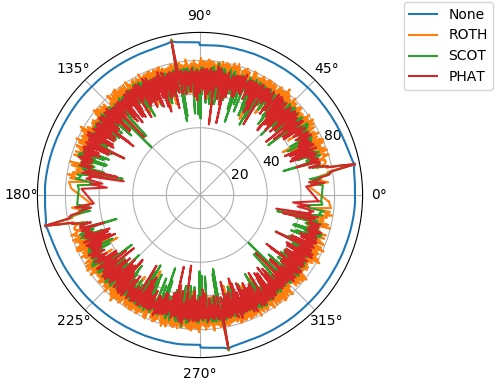
\includegraphics[width=0.9\textwidth]{Figures/GCC_20_20.png}
    \caption{Both sources at 20dB SNR}
    \label{fig:d3}
\end{subfigure}
\quad
\begin{subfigure}[b]{0.48\textwidth}
    \centering
    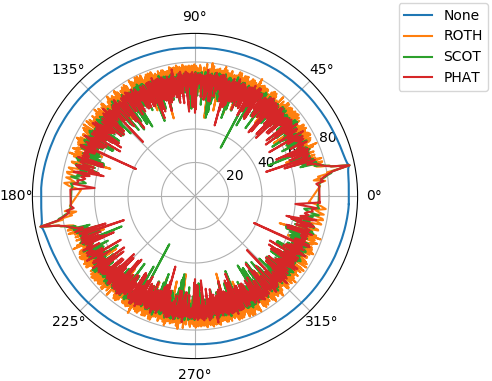
\includegraphics[width=0.9\textwidth]{Figures/GCC_0_20.png}
    \caption{S1 at 20 SNR, S2 at 0 SNR}
    \label{fig:d4}
\end{subfigure}
\caption{Figures compares different GCC algorithms for localization performance for 2 sources with various SNRs. The simulations assume 2 microphones placed 1m apart along the $0\degree-180\degree$ axis. The sampling rate is assumed to be 192kHz and speed of sound is 343m/sec. Two sources playing pink noise at different levels and located at $S_1:15\degree$ and $S_2:100\degree$ are assumed. Uncorrelated white noise is assumed to be present at the 2 microphones. No interpolation fixing is done. The level of the noise is unchanged but the level of the signal is varied to achieve the different SNRs.}
\label{fig:GCC_SIM}
\end{figure}


\subsection{Multiple pair GCC}

GCC equations described above are for a single pair of microphones only. Various algorithms have been designed that extend the GCC algorithm to multiple pairs of microphones. SRP-PHAT approach \cite{dibiase2000high} combines the steered response power (SRP) beamformer methods \cite{krim1996two} to the GCC approach. Griebel \cite{griebel2001microphone} describes a method where the \enquote{GCC functions derived from various microphone pairs are simultaneously maximized over a set of potential delay combinations consistent with candidate locations} which can be seen as a special case of SRP-PHAT where the redundant information from additional microphone pairs are utilized. \textit{Okuyama et al.} show in a 2002 study\cite{okuyama2002study} that when using a spatial array like a tetrahedron, the propagation direction of sound through the array can be determined, irrespective of the speed of sound, by using the least-squares approach. This means that for localizing sound sources outdoors, the instantaneous temperature and wind on the microphone array need not be known. Benesty \cite{benesty2004time} provides a method to fully utilize the redundant information from multiple microphone pairs to make the time-delay estimation (TDE) process more robust against distortion and also improve angular resolution. The method re-derives multi-channel cross correlation (MCCC) to apply linear interpolation on the GCC data to improve the angular resolution of localization. More recently, in \cite{liu2010continuous} the author used a motorized robot with 4 microphone arranged in a cross-formation. The algorithm uses 'de-noising' techniques such as adding a small regularization term to the denominator of the PHAT weight, which can reduce the low SNR issues surrounding PHAT. The low SNR regions can be further penalized by using reliability-weighted RW-PHAT \cite{valin2006robust}, where a-priori SNR information is used to estimate the weight to be multiplied during the PHAT computation. Eigenvalue decomposition based GCC (ES-GCC) is done by authors in \cite{hu2009estimation}. They conclude that ES-GCC produces less number of outlier locations that GCC-PHAT. Badali \cite{badali2009evaluating} compares various localization algorithms using a 8 microphone array located on a cube. The authors use hyperbolic intersection on the GCC results from multiple pairs of microphones. They conclude that if \textit{Direction Refinement} procedure is run, in which first a far-field assumption search is done and the locations are then 'refined' for near field, then the results from SRP-PHAT can be improved. But this procedure might not be relevant for far-field outdoor localization.  

The next sections will discuss some of the algorithms that are relevant for outdoor source localization and make the PHAT process more robust. 
\subsection{Steered Response Power}

Steered Response Power (SRP) source localization is a method to detect sound source locations using beamforming techniques \cite{krim1996two}. SRP is different from TDOA based methods discussed before. While the generalized cross correlation is a simple cross correlation between each pair of microphones and only outputs an estimate of the time delay, the SRP method beamforms the space around the array and computes the energy of each location beam.  It `looks' at all possible directions individually (steering) and computes the power of the signal cross correlation in that direction (beamforming). The assumption is that the cross power of the steered microphone array will be the maximum in the correct source direction. However, the computational demand for this can rise quite fast (depending on the sampling rate and the angular resolution of the beamforming), making it nearly impossible to implement in real time applications. However, its performance in difficult conditions outperforms the TDOA based methods \cite{dmochowski2007generalized}. Since real-time localization is not of primary importance for this thesis, SRP based methods can be applied. In the same fashion as the GCC method proposed to pre-filter the signal before performing the cross correlation, a PHAT weighing can be applied on the beamformed signal. This method is called SRP-PHAT. In this section, the first part discusses the basic principles behind the method whereas the second part introduces a hybrid method that improves the computational time of SRP without decreasing its robustness. 

%\subsubsection{Steered Beamformer}

The SRP method is based on a regular delay-and-sum beamformer, for a given point in space having range $\rho$, azimuth $\theta$ and elevation $\phi$ with the microphone array, the output of the beamformer is given by

\begin{equation}
    y_{\rho,\theta,\phi}(n)=\sum\limits_{m=0}^{M-1}{w_m x_m[n + f_{0,m}(\rho,\theta,\phi)]},
\end{equation}

where $x_0[n]$ is the signal received at time n, at an arbitrary microphone used as reference, $w_m$ is the amplitude weight for microphone m, and $f_{0,m}(\rho,\theta,\phi)$ is the relative delay between the reference microphone and the $m^{th}$ microphone. When far-field approximation is assumed, the range cannot be computed and the delay-and-sum beamformer output can be rewritten as follows:

\begin{equation}
    y_{\theta,\phi}(n)=\sum\limits_{m=0}^{M-1}{w_m x_m[n + f_{0,m}(\theta,\phi)]} 
\end{equation}


For $w_m=1$ (assuming perfectly omni-directional and equally sensitive microphones), the output power of the beamformer becomes

\begin{equation}
    \mathbb{E}[{y_{\theta,\phi}(n)^2}]=\sum\limits_{i=0}^{M-1}\sum\limits_{j=0}^{M-1}{R_{x_i,x_j}[f_{i,j}(\theta,\phi)]} 
    \label{eq:poweroutputbeamformer}
\end{equation}

This cross correlation is computed in the frequency domain using cross-spectrum which is then inverse fast Fourier transformed (IFFT).

\begin{equation}
    R_{x_i,x_j}(\tau)= \sum\limits_{k=0}^{N_{f}-1}{X_{i}(k)X_{j}^*(k)e^{j2\pi\frac{k}{N_{f}}\tau}}
\end{equation}

%\subsubsection{SRP Search}

The SRP method starts with a look up procedure which associates each set of angles ($\phi,\theta$) to a given set of delays between each microphone pair. For instance if we use a 1$\degree$  resolution, the SRP method associates 360*360=129600 angular positions to corresponding delays. The cross correlations of the signals received at the different microphone pairs combinations possible are then computed. For a given position ($\phi,\theta$), the output of the SRP search is simply the sum of the cross correlation at each time delay found relative to each pair of microphone. It corresponds to the power output of the beamformer defined in Eq. \ref{eq:poweroutputbeamformer}. 
\begin{equation}
    S_{SRP}(\theta,\phi)=\sum\limits_{i=0}^{M-1}\sum\limits_{j=0}^{M-1}{R_{x_i,x_j}[f_{i,j}(\theta,\phi)]}
\end{equation}

\begin{figure}[H]
    \centering
    \begin{subfigure}[t]{0.5\textwidth}
    \centering
    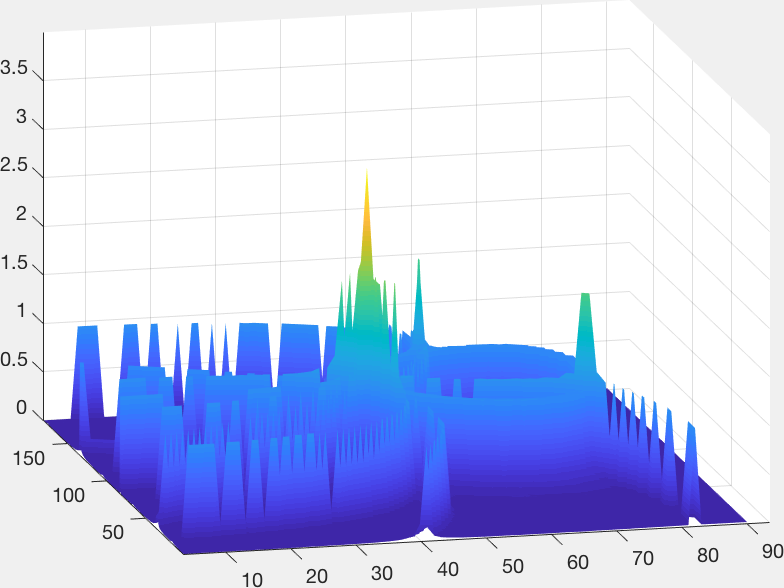
\includegraphics[width=0.9\textwidth]{Figures/viewside.png}
    \caption{SRP map}
    \label{fig:viewsidesrp}
\end{subfigure}%
\begin{subfigure}[t]{0.5\textwidth}
    \centering
    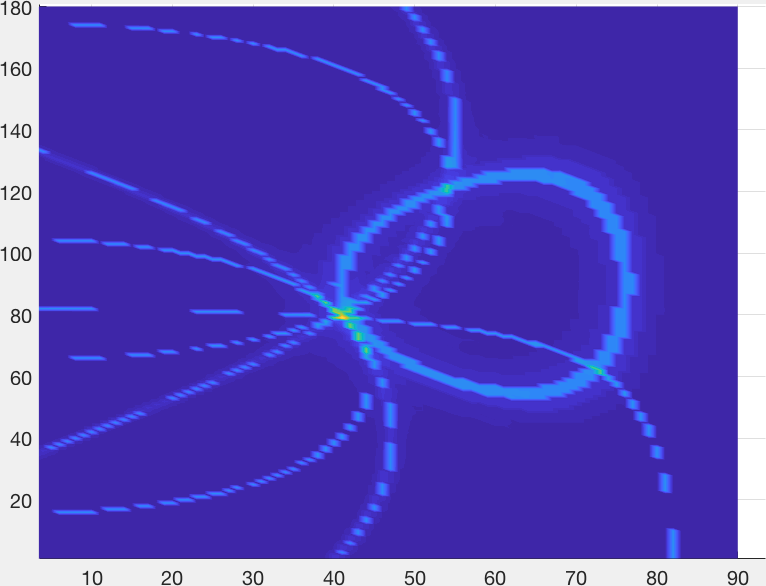
\includegraphics[width=0.9\textwidth]{Figures/topview.png}
    \caption{SRP heat map}
    \label{fig:topviewsrp}
\end{subfigure}
\caption{Power mapping simulation of source localized using SRP-PHAT algorithm in noiseless, free-field situation. For the simulation, first a 4-channel wav file is created such that the channels contain the same pink noise but delayed between each other. The delays are such that the source would be ideally located at azimuth $80\degree$ and elevation $40\degree$ when localized by a 1m aperture tetrahedral array. SRP-PHAT is then applied on the wav file and power received from different angles (beams) is computed and plotted. As can be seen the algorithm was able to localize the source in these ideal conditions fairly correctly.}
\end{figure}

The SRP method estimates the source location ($\hat{\phi},\hat{\theta}$) after creating the SRP search space such that

\begin{equation}
    \hat{\phi},\hat{\theta}=\argmax_{\phi,\theta}S_{SRP}(\phi,\theta)
\end{equation}

%\subsubsection{Premapping the delays to potential sources locations}

The classical SRP search beamforms sequentially the 3D space and locations [($\phi_{1},\theta_{1}$), ($\phi_{2},\theta_{2}$), ... ,($\phi_{x},\theta_{x}$)] which might be associated with the same relative delay $\tau_{1}$ (in case of a uniform linear microphone array). The cross correlation at delay $\tau_{1}$ is then computed $x$ times, which leads to the same results for each [($\phi_{1},\theta_{1}$), ($\phi_{2},\theta_{2}$), ... ,($\phi_{x},\theta_{x}$)] positions, leading to numerous useless cross correlation computations. In \cite{dmochowski2007generalized} the authors propose an improvement on the SRP search algorithm by pre-mapping the relative delays to their corresponding set of locations. Instead of proceeding to a sequential search in the 3D space, a search on the possible relative delays is considered. The possible delays between individual microphone pairs are already known based on the array geometry and can be stored in memory. The cross correlations are calculated for each delay subset and related to a set of potential source location in space in the final steps of the algorithm. Note that the computational cost gain can be immense depending on the number of microphones (the more the microphones, the greater the gain), the aperture size (the smaller the microphone array the more angles are associated with the same time delay) or the sampling rate (again the smaller the sampling rate the more angles are associated with the same time delay). In GCC methods this issue was taken care of by interpolation, where the microphone pair end-side localization had poor resolution (Fig. \ref{fig:res_diff}). 

The method can be easily extended to SRP-PHAT, where pre-filtering the signal beforehand by using PHAT introduces a function $\psi_{ij}$ in the cross correlation

\begin{equation}
    R_{x_i,x_j}(\tau)= \sum\limits_{k=0}^{N_{f}-1}{\psi_{ij}(k) X_{i}(k)X_{j}^*(k)e^{j2\pi\frac{k}{N_{f}}\tau}}
\end{equation}
where
\begin{equation}
    \psi_{ij}(k) = \frac{1}{|{X_{i}(k)X_{j}^*(k)}|}
\end{equation}

\subsubsection{Simulations}

Two identical sound sources are placed in the far field. A tetrahedral array with equal spacing between microphones of 1 meter is receiving the two sources. The sound received at the sources are 3 seconds of two different pink noises with respective DOA $\tetha_{1}=120\degree$, $\phi_{1}=40\degree $ and $\tetha_{2}=150\degree $ , $\phi_{2}=75\degree $. Waves are propagating in free field where no reflections and no noise is added to the microphones. The SRP maps are computed and displayed in the figure \ref{fig:coherent2pinknoise}. Source 2 is placed at a problematic angle for the tetrahedral array, detection errors are discussed in section \ref{sec:detection}. Error probability increases as the source DOA approach the angle of the axis drawn by pairs of microphones (end-side).

\begin{figure}[H]
    \centering
    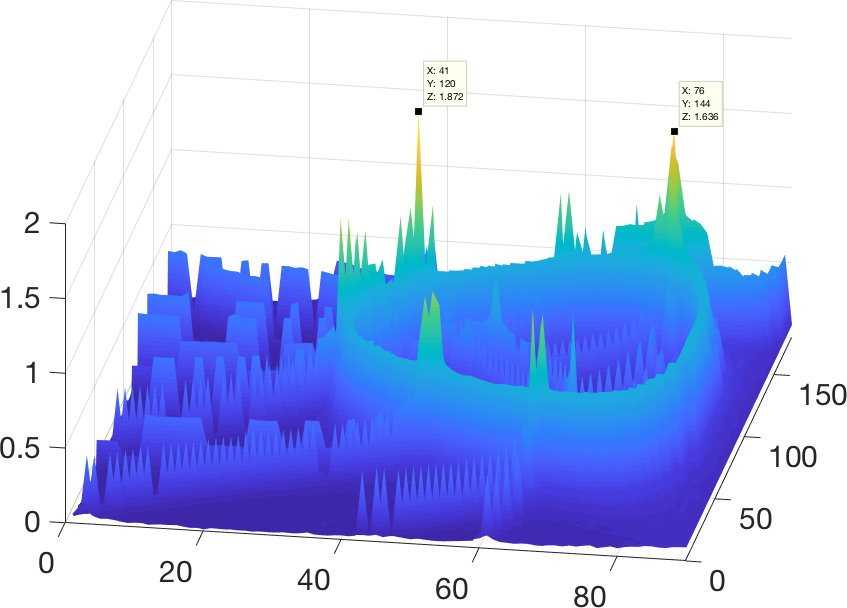
\includegraphics[width=1\textwidth]{Figures/2pinknoisesrpphat.png}
    \caption{SRP-PHAT simulation with 2 sound sources localized using a tetrahedral array}
    \label{fig:coherent2pinknoise}
\end{figure}

\subsubsection{Localization errors} \label{sec:detection}

Two pairs of microphones are considered, the axes drawn by the two pairs is plotted (extended) in figure \ref{fig:locerrortetra}. The two axes form respective angles of $45\degree$ and $60\degree$ with the horizontal axis. Plane waves with DOA between $45\degree$ and $60\degree$ will cross the two pairs of microphones at an angle close to the respective end-sides of the pairs. As shown in figure \ref{fig:errorsimulation1} maximum errors arise in the simulation for DOA contained in between $45\degree$ and $60\degree$. For a tetrahedral array, this can be seen as the 3d space created by extending the arms connecting the microphones. 

\begin{figure}[H]
    \centering
    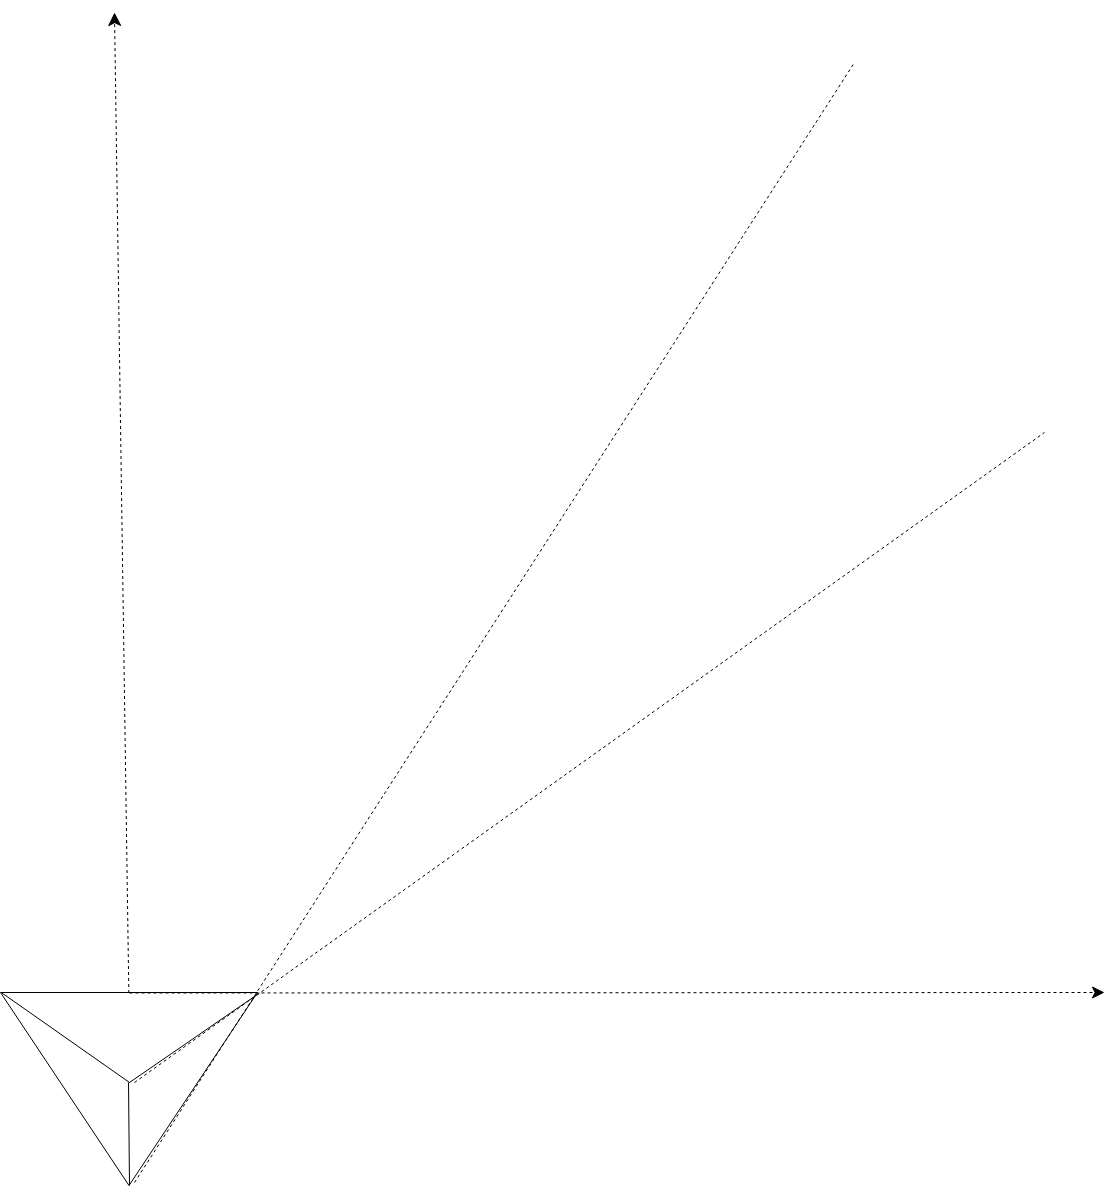
\includegraphics[width=0.9\textwidth]{Figures/locerrors.png}
    \caption{Axis drawn by 2 pairs of microphones}
    \label{fig:locerrortetra}
\end{figure}

\begin{figure}[H]
    \centering
    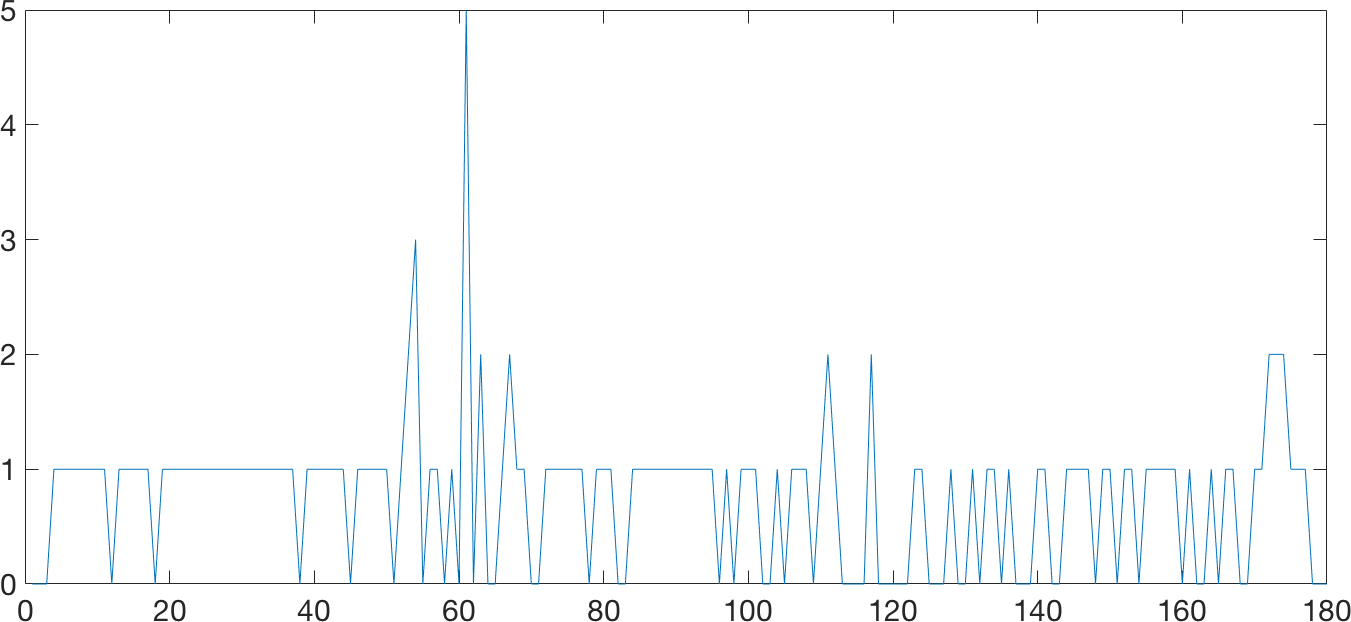
\includegraphics[width=0.9\textwidth]{Figures/errorphinointerpolationandrounding.png}
    \caption{Simulation errors with no interpolation}
    \label{fig:errorsimulation1}
\end{figure}

\subsection{Hybrid SRP-PHAT}

Peterson \cite{peterson2005hybrid} describes a novel approach for sound localization using a two stage approach in order to reduce the computational load. The first stage roughly identifies the sources locations while the second stage is a modified version of the SRP-PHAT algorithm that only performs a grid search around the estimated location from the first stage.  The method is well suited for near-field localization using large aperture array which is not our requirement but the idea can be adapted in the case of far-field sound localization. Section \ref{sec:TDOA} gives an introduction to TDOA based localization and introduces the cone approximation for the far-field. The idea of the hybrid approach is to do a classical GCC-PHAT estimation to get the relative delays between the sensors. The delays estimates are used to derive the cone intersections which give a location estimate which is then input into a SRP-PHAT algorithm where the search region is constrained around the location estimates. A system overview of the algorithm is given in figure \ref{fig:hybridalgo}.

\begin{figure}[H]
    \centering
    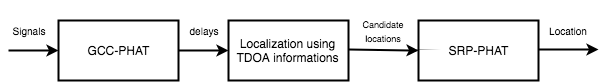
\includegraphics[width=1\textwidth]{Figures/hybridalgo.png}
    \caption{Simplified block diagram of the Hybrid algorithm}
    \label{fig:hybridalgo}
\end{figure}

\subsection{Improvements on SRP}

In \cite{salvati2017exploiting} the author proposes a method to improve the computational efficiency and coherence of the grid search using discreet sampling information where the method is called geometrically sampled grid (GSG). \cite{do2007real} uses Stochastic Region Contraction(SRC) to reduce the computational time of the search. \cite{salvati2014incoherent} introduces an incoherent Frequency Fusion based on a normalized arithmetic mean (NAM) which improves the localization performance of SRP, MVDR and MUSIC. Paper \cite{salvati2015frequency} introduces a SRP weighted MVDR, which combines machine learning power to the noise resilience of the MVDR beamformer, the method is improved in \cite{salvati2016use} by using SVM training. SRP-WMVDR is proved to be much more resilient to noise and better than SRP-PHAT for SNR up to 0. All of those papers uses a microphone array composed of mostly more than 8 microphones. Few experiment data are available for the case of 4 microphones and none for the case of a tetrahedral array, whereby a ULA is mostly used for the different test methods.



\section{Robust solution: SRP-PHAT}
\subsection{Behavior and error sources}
\subsubsection{Array response}
Beamforming techniques for sound localization have been study intensively over the last decades. The main drawback of the conventional beamforming are the side lobes in the localization results. If SRP-PHAT algorithm is applied to a tetrahedral array and cross-correlations values at different delays are summed by the beamformer (Eq. \ref{eq:srpSum}), subsidiary peaks can appear in the energy map at DOAs that don't correspond to the incident plane wave DOA. Those peaks in the SRP-PHAT energy map can mask real sources or even add up to other peaks from other sources, thus display a fake source. Deconvolution methods remove those peaks to reveal the correct peak. The algorithms for deconvolution are based on the point spread function, which is the response of the array to a point source. 
%For far-field, this means a plane wave incident with a particular DOA on the microphone array. In transfer function terms, the array response is `deconvolved' from the final energy map. 
%While this problem has motivated the creation of new beamformers {!!CITATION!!}, the problem lies in the method itself.
%New classes of algorithms have been developed to deconvolve the noise signals from the desired steered signal such as CLEAN \cite{sijtsma2007clean} and DAMAS \cite{brooks2006deconvolution}.
%DAMAS was acknowledged a major breakthrough in array processing. At first research was mainly focused on aeroacoustic for the development of near-field sound localization system but it seems that a new enthusiasm has taken over scientists trying to solve other sound localization problems. 
%While the DAMAS method is mainly designed for near field measurements in the range of the array aperture size, a new deconvolution method has been proposed [\cite{zhao2015large}, \cite{zhao2017large}] where a small aperture array is used to measure source signal in the far field. The principle behind point spread function is discussed in the following section. Then a review of the underlying principles of the main deconvolution algorithms is given, and finally a specific method for coherent and incoherent sources localization is discussed.
A perfect array will detect a point precisely at the actual source location and nothing elsewhere. This, however, is not the general case. For example, given a single pair of microphones, and assuming far-field incidence, the only information that can be concluded from a single point source is the angle of incidence on the array. This angle is a vector combination of source azimuth and elevation. This leads to a circle around the array where the source might be located (circular maximum peak). This circle is the base of the cone resulting from the cone approximation discussed previously.

%\begin{figure}[H]
%    \centering
%    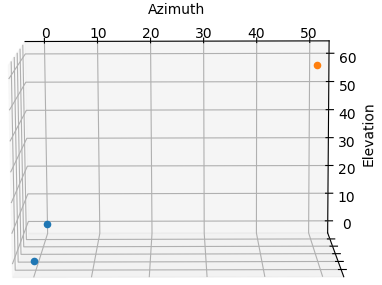
\includegraphics[width=0.98\textwidth]{Figures/2mic1src.png}
%    \caption{Figure depicts a source located at $50\degree$ azimuth and $60\degree$ elevation (orange dot). Two microphones (blue dots) will be used to localize the source.}
%    \label{fig:2mic1srcPos}
%\end{figure}

\begin{figure}[H]
    \centering
    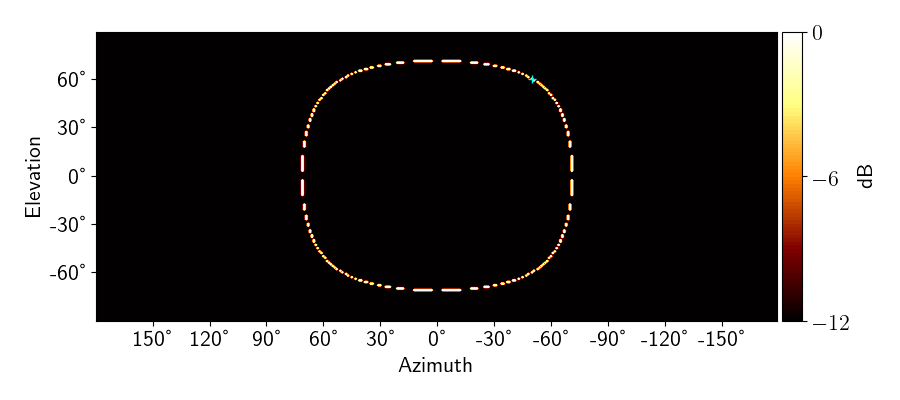
\includegraphics[width=0.8\textwidth]{Figures/2mic1srcRes.png}
    \caption{SRP-PHAT is run to localize a single point source with 2 microphones. The source is localized to a circle. The red dot indicates the actual source location.}
    \label{fig:2mic1src}
\end{figure}

If three microphones are placed in a horizontal equilateral triangle, we get three circles (three possible pairs of microphones) from localization. The maximum peak occurs at 2 locations with azimuth=50$\degree$ and elevation=$\pm 60\degree$.
\begin{figure}[H]
    \centering
    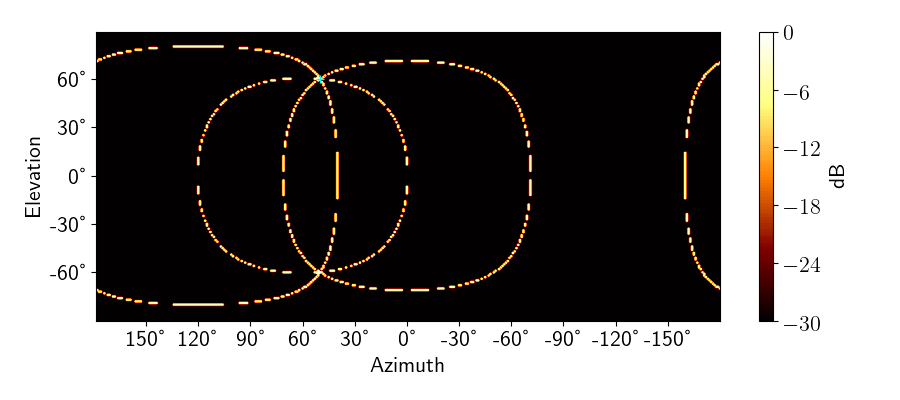
\includegraphics[width=0.8\textwidth]{Figures/3mic1srcRes.png}
    \caption{SRP-PHAT is run to localize the source with 3 microphones.}
    \label{fig:3mic1src}
\end{figure}

For a tetrahedral array, the point spread function is a combination of circles from the 6 possible microphone pairs. This time the main peak occurs at exactly one point. However, since only 3 pairs out of the 6 are linearly independent (Eq. \ref{Eq:linearDep}), the localization should really be done considering only 3 of those pairs. The result in shown in fig. \ref{fig:4mic1srcInd}
\begin{figure}[h]
    \centering
    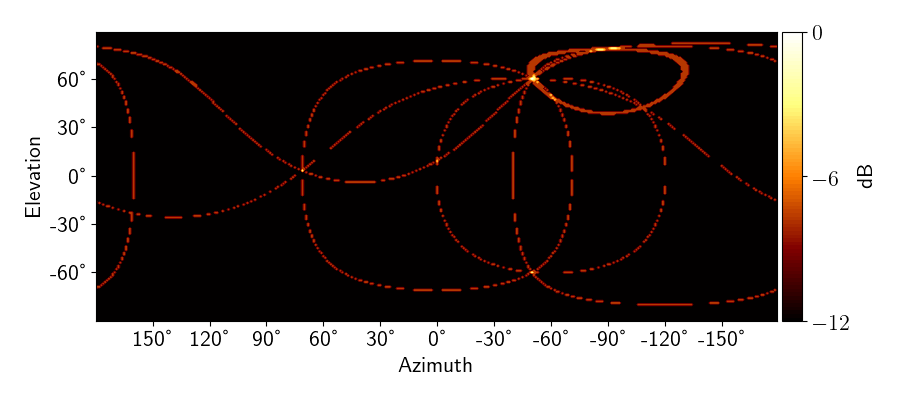
\includegraphics[width=0.8\textwidth]{Figures/4mic1srcRes.png}
    \caption{SRP-PHAT is run to localize the source with a tetrahedral array.}
    \label{fig:4mic1src}
\end{figure}


\begin{figure}[h]
    \centering
    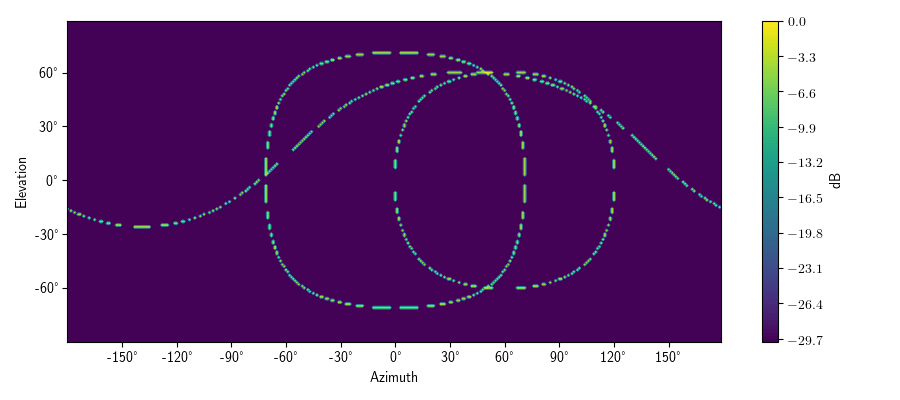
\includegraphics[width=0.8\textwidth]{Figures/Ind4mic1src.png}
    \caption{SRP-PHAT is run to localize the source with a tetrahedral array but only linearly independent microphone pairs are considered}
    \label{fig:4mic1srcInd}
\end{figure}
The result in fig. \ref{fig:4mic1src} is applicable only in ideal conditions (zero noise, no reflections and perfectly planar propagation). The localization result obtained in noisy conditions, is depicted in fig. \ref{fig:4mic1srcNoisy}. Note that the color bars for the figures depicted are of the same color scale. The localization performance deteriorates as the SNR drops. The result is similar to the results for PHAT with 2 microphones discussed earlier as the underlying process in SRP-PHAT is still PHAT. As can be seen in the figure, even in ideal conditions, the localization results contain many peaks of varying heights. This is due to summing the cross-correlation responses of a non-linear array (Eq. \ref{eq:srpSum}). If the array were linear, the localization circles from each pair would all overlap completely. In case of a tetrahedral array, the localization circles from the possible microphone pairs are not co-planar. This is because all the edges of a tetrahedron point in the different directions. The obvious problem here is multi-source detection. If multiple sources are playing at different levels, how do we determine if a detected peak is a real source or a relic from another higher level source? The methods to do so form the basis of deconvolution methods. A simple deconvolution approach could be to penalize sources detected only by a subset of the microphone pair combinations. This could be done by taking a product and not a sum in Eq. \ref{eq:srpSum}. This way, if a peak is caused by a single localization circle, the cross-correlation values from other microphone pairs would be close to zero, and thus would scale the false peak down. The localization results from this are given in fig. \ref{fig:4mic1srcNoisyProd}. Fig. \ref{fig:4mic2srcNoisyCompare} compares the localization result for two equally loud sources, this time located at (azimuth, elevation) = (-20, -30) and (50, 60), with normal SRP-PHAT and product-SRP-PHAT. The results are convincingly better for simulations.  

\begin{figure}[H]
    \centering
    \begin{subfigure}[b]{0.96\textwidth}
    \centering
    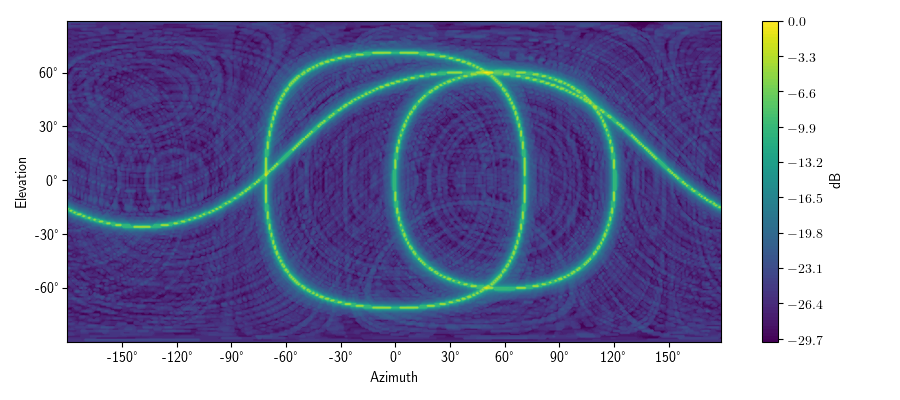
\includegraphics[width=0.8\textwidth]{Figures/Ind4mic1src20.png}
\end{subfigure}
\vskip \baselineskip
\begin{subfigure}[b]{0.96\textwidth}
    \centering
    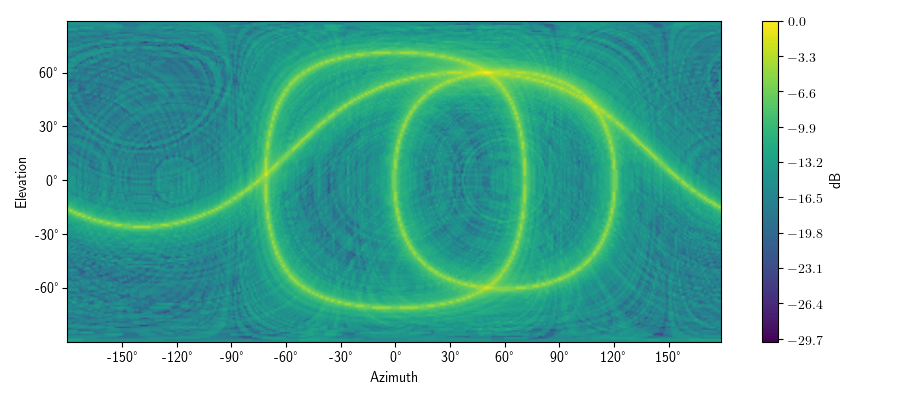
\includegraphics[width=0.8\textwidth]{Figures/Ind4mic1src6.png}
\end{subfigure}
\vskip \baselineskip
\begin{subfigure}[b]{0.96\textwidth}
    \centering
    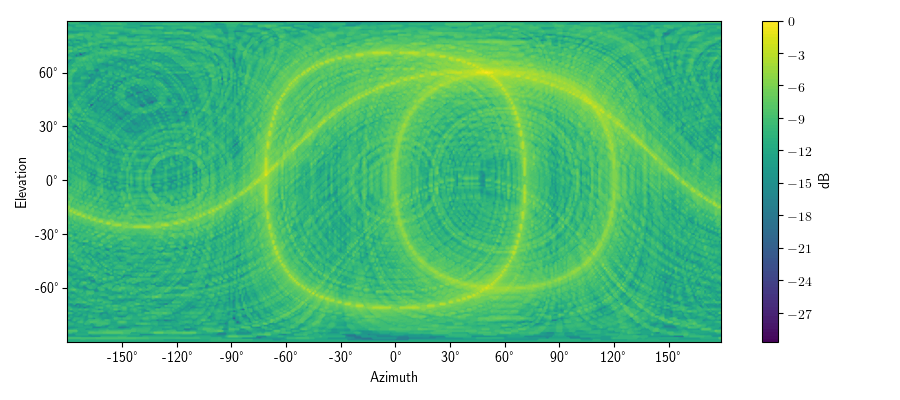
\includegraphics[width=0.8\textwidth]{Figures/Ind4mic1src0.png}
\end{subfigure}
\vskip \baselineskip
\begin{subfigure}[b]{0.96\textwidth}
    \centering
    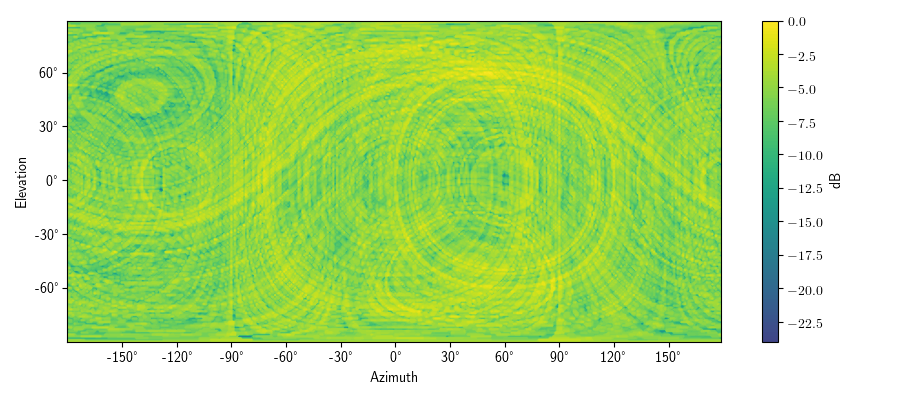
\includegraphics[width=0.8\textwidth]{Figures/Ind4mic1srcNeg6.png}
\end{subfigure}
\caption{Figures depict from top-to-bottom SRP-PHAT localization results with SNR = 20dB, SNR = 6dB, SNR = 0dB, SNR = -6dB}
\label{fig:4mic1srcNoisy}
\end{figure}

 \begin{figure}[H]
    \centering
    \begin{subfigure}[b]{0.96\textwidth}
    \centering
    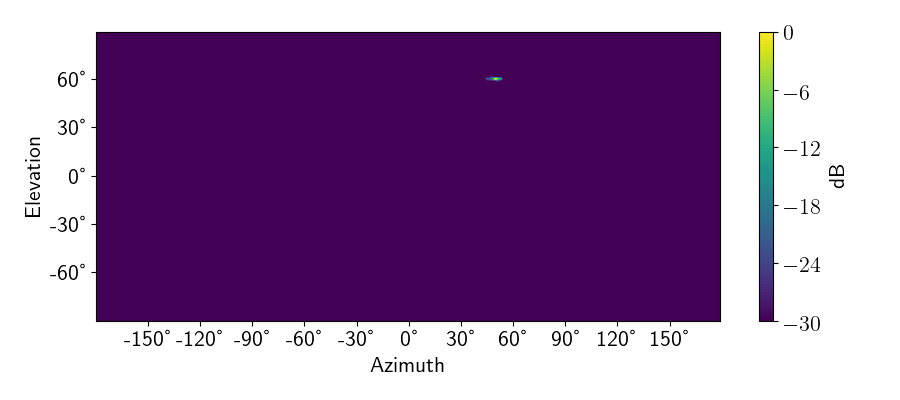
\includegraphics[width=0.8\textwidth]{Figures/Ind4mic1srcProd20.png}
\end{subfigure}
\vskip \baselineskip
\begin{subfigure}[b]{0.96\textwidth}
    \centering
    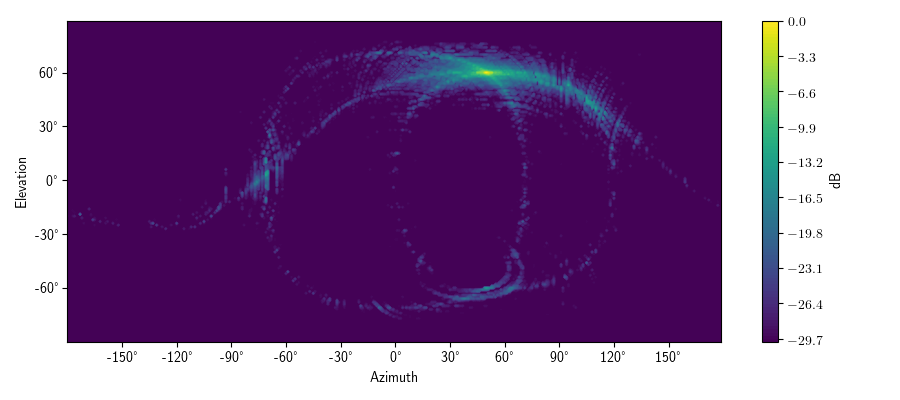
\includegraphics[width=0.8\textwidth]{Figures/Ind4mic1srcProd6.png}
\end{subfigure}
\vskip \baselineskip
\begin{subfigure}[b]{0.96\textwidth}
    \centering
    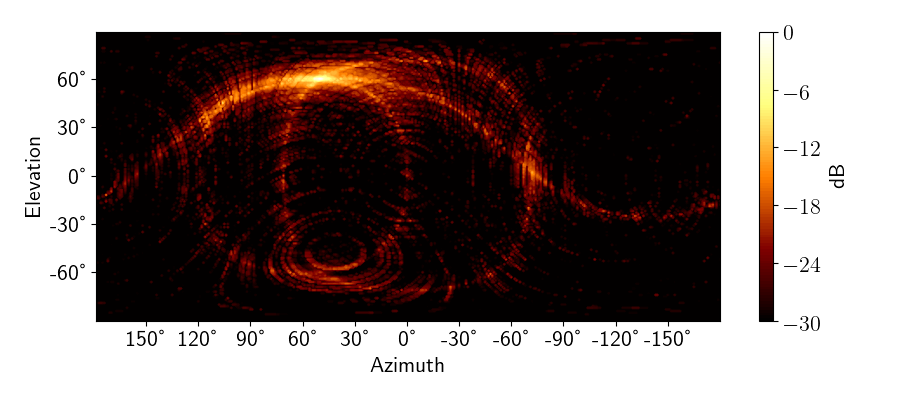
\includegraphics[width=0.8\textwidth]{Figures/Ind4mic1srcProd0.png}
\end{subfigure}
\vskip \baselineskip
\begin{subfigure}[b]{0.96\textwidth}
    \centering
    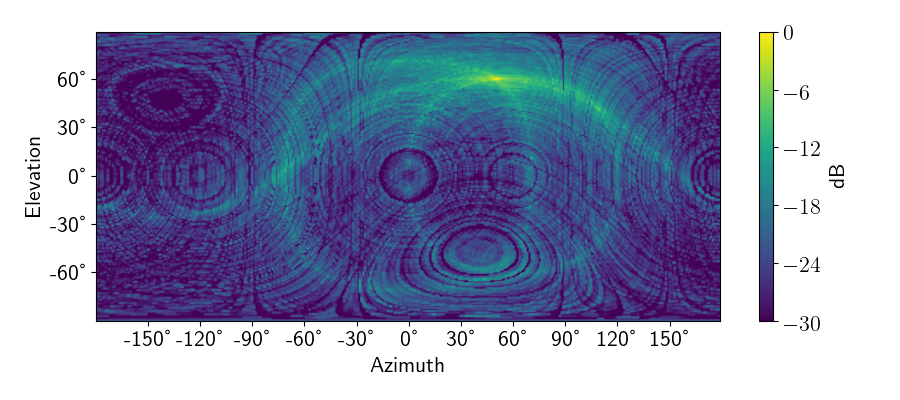
\includegraphics[width=0.8\textwidth]{Figures/Ind4mic1srcProdNeg6.png}
\end{subfigure}
\caption{Figures depict from top-to-bottom product-SRP-PHAT localization results  with SNR = 20dB, SNR = 6dB, SNR = 0dB, SNR = -6dB}
\label{fig:4mic1srcNoisyProd}
\end{figure}

 \begin{figure}[H]
    \centering
    \begin{subfigure}[b]{0.96\textwidth}
    \centering
    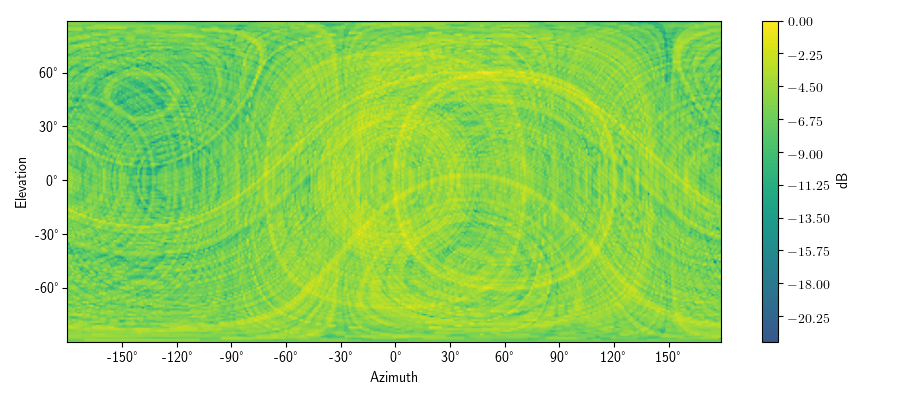
\includegraphics[width=0.8\textwidth]{Figures/Ind4mic2srcSumNeg6.png}
\end{subfigure}
\vskip \baselineskip
\begin{subfigure}[b]{0.96\textwidth}
    \centering
    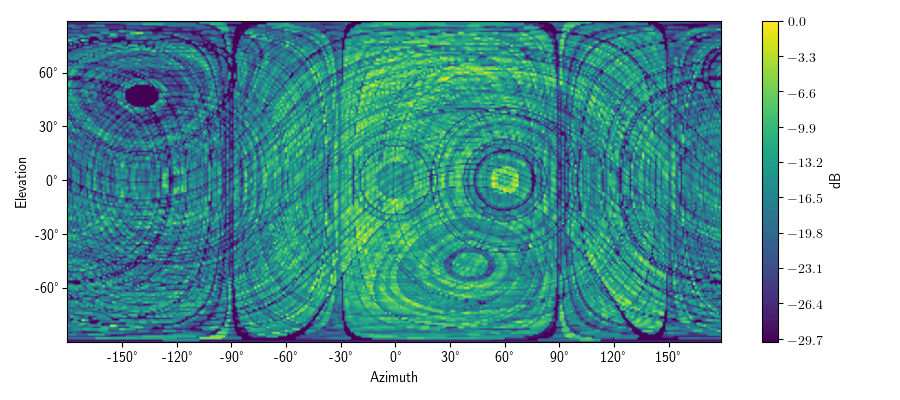
\includegraphics[width=0.8\textwidth]{Figures/Ind4mic2srcProdNeg6.png}
\end{subfigure}
\caption{Figures depict from localization results with normal SRP-PHAT (top) and product-SRP-PHAT (bottom)}
\label{fig:4mic2srcNoisyCompare}
\end{figure}

\begin{figure}[H]
    \centering
    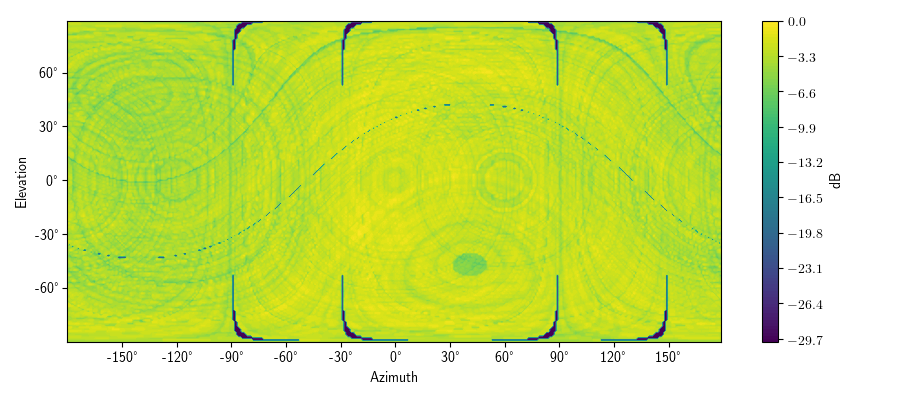
\includegraphics[width=0.8\textwidth]{Figures/Ind4mic2srcProdNeg6Div.png}
    \caption{Product-SRP-PHAT is run to localize 2 sources located at (azimuth, elevation) = (-20, -30) and (50, 60) with a tetrahedral array. The result is divided by 3 and normalized before visualization to maintain the level difference between the different sources.}
    \label{fig:4mic2srcNoisyDiv}
\end{figure}

The drawback of using product-SRP-PHAT is that the sound level difference between the different sound sources is lost. In normal SRP-PHAT, the array magnitude response at a particular azimuth and elevation could be averaged over all microphone pair combinations. Then the level difference between 2 sources is maintained. In product-SRP-PHAT this would not be the case. However if it is assumed that a particular source will have similar magnitude response for all microphone pairs (which is not a strong assumption in far-field), then taking the cubic root of multiplied power from the possible microphone pairs, the level difference can be maintained. When plotted on dB scale, that means a simple division by 3 depicted in fig. \ref{fig:4mic2srcNoisyDiv}. Since the division has the effect of reducing the dB difference between the noise floor and the main peak, the result deteriorates.

\begin{figure}[H]
    \centering
    \begin{subfigure}[b]{0.96\textwidth}
    \centering
    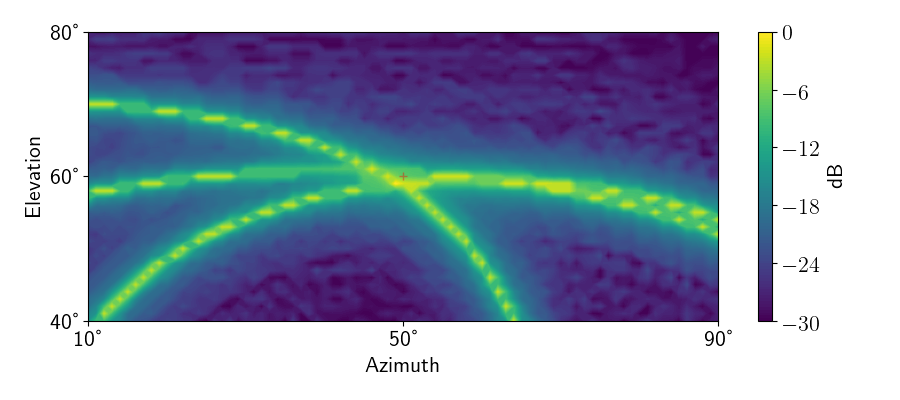
\includegraphics[width=0.8\textwidth]{Figures/Ind4mic1srcSum0deg.png}
\end{subfigure}
\vskip \baselineskip
\begin{subfigure}[b]{0.96\textwidth}
    \centering
    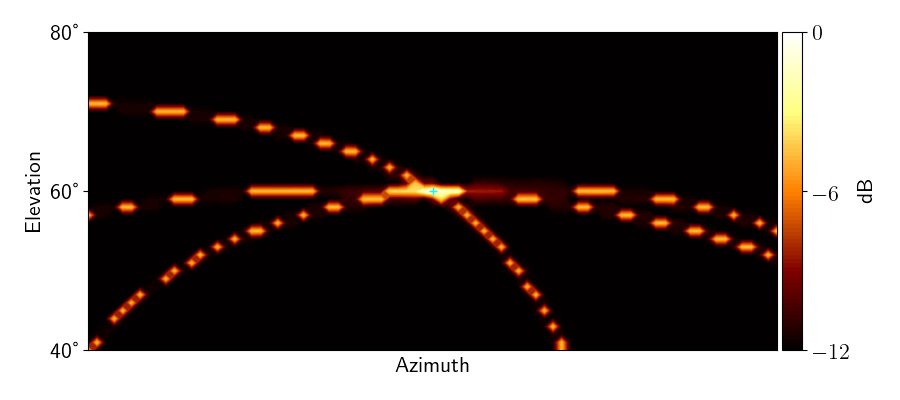
\includegraphics[width=0.8\textwidth]{Figures/Ind4mic1srcSum20deg.png}
\end{subfigure}
\vskip \baselineskip
\begin{subfigure}[b]{0.96\textwidth}
    \centering
    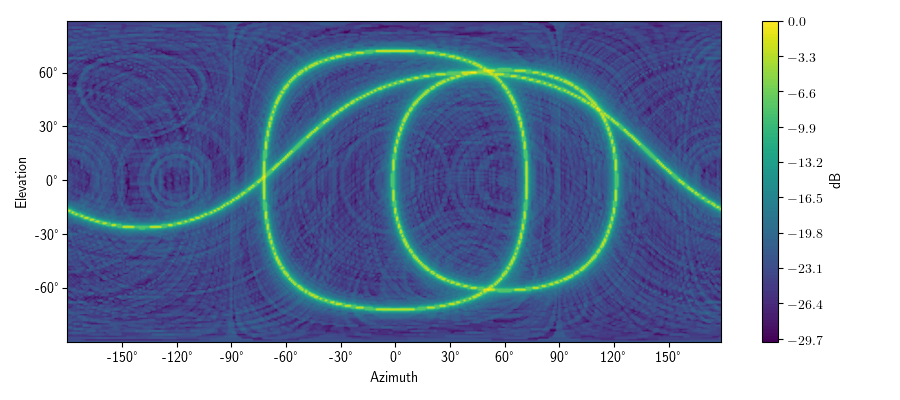
\includegraphics[width=0.8\textwidth]{Figures/Ind4mic1srcSum40deg.png}
\end{subfigure}
\caption{Figures depict from top-to-bottom SRP-PHAT localization results with at temperatures of $0\degree C$, $20\degree C$ and $40\degree C$. SNR = 20dB for every case.}
\label{fig:4mic1srcTemp}
\end{figure}

\subsubsection{Effect of temperature}
Temperature affects the speed of sound and thus affects the delay time between the microphone pairs. During measurement, if it is assumed to be room temperature, this could lead to errors in the localization results. Fig.\ref{fig:4mic1srcTemp} depicts the effect of temperature on localization results, where wave files received by the tetrahedral microphone array at temperatures of $0\degree C$, $20\degree C$ and $40\degree C$ are simulated. Then the localization is run assuming the speed of sound to be 343m/sec in every case. As can be seen in the figure, an error in recording temperature has the effect of `de-focusing' the main peak. This could lead to even great localization errors if naive deconvolution algorithms (like the product-SRP-PHAT) are then directly applied to the result. 

\begin{figure}[H]
    \centering
    \begin{subfigure}[b]{0.96\textwidth}
    \centering
    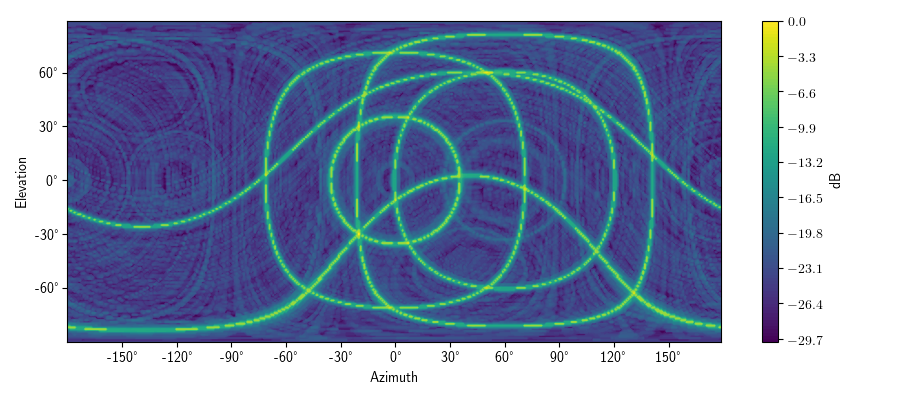
\includegraphics[width=0.8\textwidth]{Figures/Ind4mic1srcSumWind0.png}
\end{subfigure}
\vskip \baselineskip
\begin{subfigure}[b]{0.96\textwidth}
    \centering
    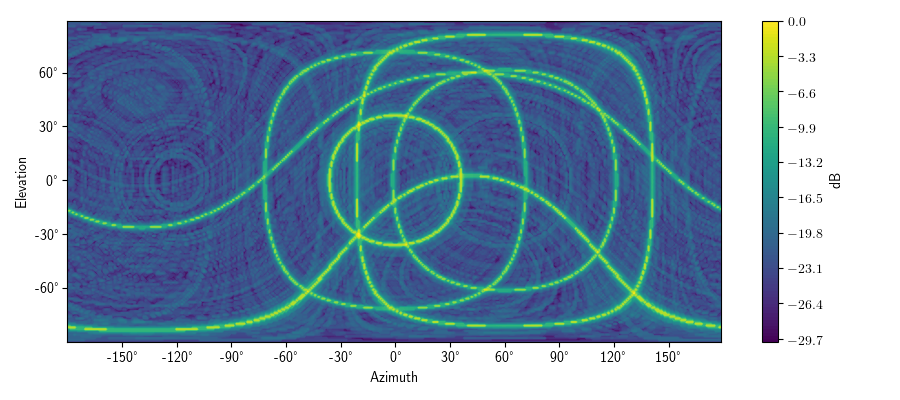
\includegraphics[width=0.8\textwidth]{Figures/Ind4mic1srcSumWind10.png}
\end{subfigure}
\vskip \baselineskip
\begin{subfigure}[b]{0.96\textwidth}
    \centering
    \includegraphics[width=0.8\textwidth]{Figures/Ind4mic1srcSumWind20.png}
\end{subfigure}
\caption{Figures depict from top-to-bottom SRP-PHAT localization results with wind of $0 m/sec$, $10 m/sec$ and $20 m/sec$. 2 sources located at (azimuth, elevation) = (-20, -30) and (50, 60) are localized with at wind (azimuth,elevation) = (50,0) and SNR = 20dB for every case.}
\label{fig:4mic2srcWind}
\end{figure}

\subsubsection{Effect of wind}
Wind speed effects the speed of sound in the direction of propagation. Delays between different array pairs would be affected depending on where the SRP search is looking and from what direction the wind is blowing. If wind blows perpendicular to the direction of propagation of the sound from the source, then it does not affect the localization. In case of multiple sources, the extent of errors due to wind will depend on the source location. Assuming wind to be blowing level (horizontally), wind direction can be described by its magnitude in m/sec and its azimuth. Fig.\ref{fig:4mic2srcWind} depicts the effect when localizing two equally loud sources without any wind correction, located at (azimuth, elevation) = (-20, -30) and (50, 60) for various conditions.

\subsubsection{Effect of ground reflections}
Sound received from a far-field sound source consists of the plane wave and the spherical wave component (Eq. \ref{Eq:GroundWave}). The plane wave components is the only component simulated so far above. The ground wave which is the spherical wave component needs to be considered as well. It is the contribution of the image created by the source with the ground. The location of this reflected sound is in vicinity of the image and depends on the smoothness of the ground material. Its magnitude depends on the magnitude of absorption of sound by the ground. Rudimentary simulations for a source located at $(\theta,\phi)$ can be made assuming sound sources located at $(\theta,-\phi)$ and $(\theta,0)$. Fig. \ref{fig:4mic1srcRef} shows the localization results with the same source located at those locations. More complex reflections are not currently planned for simulation purposes.

\begin{figure}[H]
    \centering
    \includegraphics[width=0.8\textwidth]{Figures/Ind4mic1srcSumRef.png}
    \caption{SRP-PHAT is run to localize a source located at (azimuth, elevation) = (50, 60). The source is also copied at locations (50,0) and (50,-60).}
    \label{fig:4mic1srcRef}
\end{figure}
\subsection{Deconvolution old part}

\subsubsection{CLEAN}

CLEAN is an algorithm used to remove the influence of the point spread function (PSF) on the beamformed result. It is possible to remove the side lobes of the beamformer and get a more accurate localization, but it requires many microphones. CLEAN-SC is an extension of the algorithm for the case of coherent sources, it performs the deconvolution in the frequency domain which usually assumes a shift-invariant PSF. A deconvolution technique in the time domain was developed named TIDY (add reference).

\subsubsection{DAMAS}

Conventional beamforming produces an output that is dependent on array geometry, size, source distance, and frequency. DAMAS removes those array-dependent beamforming characteristics from the output to give an explicit and non ambiguous source localization and level. The DAMAS use the steering vector $\hat{e}$ of the array defined in section.. and formulates that the output of a standard beamformer with $m_{0}$ microphones can be written as:

\begin{equation}
    Y=\frac{\hat{e}^{T}\hat{G}\hat{e}}{m_0^2}
    \label{eq:DAMASoutputbeamformer}
\end{equation}
where $\hat{G}$ is the Cross Spectral Matrix (CSM) given by
\begin{equation}
\hat{G}=
    \begin{bmatrix} 
      G_{11} & G_{12} & \cdots & G_{1m_{0}}\\
      \vdots &  G_{22} &       &  \vdots\\
      \vdots &         & \ddots &  \vdots\\
      G_{m_{0}1} &     &       &  G_{m_{0}m_{0}}\\
    \end{bmatrix}  
\end{equation}
$G_{mm'}$ is the cross spectrum between microphone m  and m'. It is computed by taking the FFT of the pressure recording $p^{*}_{mk}(t)$ and $p_{m'k}(t)$ averaged over K data blocks. $w_{s}$ is a weight filter like Hamming window.
\begin{equation}
    G_{mm'}=\frac{2}{Kw_{s}T}\sum\limits_{k=0}^{K}[P^{*}_{mk}(f,T)P_{m'k}(f,T)]
\end{equation}

Pressure at the two microphones $p^{*}_{mk}(t)$ and $p_{m'k}(t)$ can be split to form two terms accounting for the amplitude of the signal and the steering vector, such that the cross spectrum for a single source can be written as the product of the squared pressure with the cross spectrum of the steering vectors K:

\begin{equation}
\hat{G}_{n}= X_{n} 
\begin{bmatrix} 
      e_{1}^{-1}^{*}e_{1}^{-1} & e_{1}^{-1}^{*}e_{2}^{-1} & \cdots &   e_{1}^{-1}^{*}e_{m_{0}}^{-1}\\
      e_{2}^{-1}^{*}e_{1}^{-1} & e_{2}^{-1}^{*}e_{2}^{-1} &       &  \vdots\\
         &     & \ddots &   \vdots\\
       &     &   &   e_{m_{0}}^{-1}^{*}e_{m_{0}}^{-1}\\
    \end{bmatrix}_{ n}= X_{n}.K 
\end{equation}   

DAMAS assumes that the total CSM is the sum of all of N sources CSM
\begin{equation}
    \hat{G}=\sum_{n}\hat{G}_{n}
\end{equation}  

Therefore, the output of the output of the beamformer in equation \ref{eq:DAMASoutputbeamformer} can be rewritten as

\begin{equation}
    Y(\hat{e})=\frac{\hat{e}^{T}\sum_{n}\hat{G}_{n}\hat{e}}{m_0^2}=\frac{\hat{e}^{T}\sum_{n}X_{n}K\hat{e}}{m_0^2}=\sum_{n}\frac{\hat{e}^{T}K\hat{e}}{m_0^2} X_{n}
\end{equation}

The left term of the product being rewrote as the product of the propagation matrix A with $X_{n}$.
\begin{equation}
    A=\sum_{n}\frac{\hat{e}^{T}K\hat{e}}{m_0^2}
\end{equation}
Giving the following linear equation
\begin{equation}
    Y = A X_{n}
\end{equation}


\subsubsection{DAMAS-C}

As the classical array beamforming, it relies on the following assumption: noise regions under study are distributions of statistically independent sources. Therefore if coherent sources a present it can produce a distorted output. Therefore an extention to DAMAS has been developped to deal with the coherent sources case.


\subsubsection{Multiposition-DAMAS}

A method has been used to scan a large 2D plane using a small aperture array at several position. It is based on DAMAS and gave good resolution once again there is a lot of microphone on the array. The article proposes to solve the DAMAS problem using Covariance Matrix Fitting.






\subsubsection{Discussion}

Deconvolution methods are of great interest as they recover the source level and position at once. It is computationally heavy but it gives improves results over the classial beamforming method. The research current focus is on planar microphone array and nobody has applied deconvolution to tetrehedral arrays also the drawback of such as system is that they seem to relie on a high number of microphones, the low number of microphones case has not been investigated in term of robustness and multi sources.
Might be useful for coherent sources mapping (ground effect), it also solve the SPL. It is a good method designed for a moving microphone array. Drawback are that the bigger area to investigate, the bigger the aperture of the array must be (For one position). If there is several positions used to measure then it's ok.  More on that soon
\subsection{Blind Deconvolution}
%\subsection{Eigenvalues decomposition algorithm}

\subsection{Hybrid SRP-PHAT}

Peterson \cite{peterson2005hybrid} describes a novel approach for sound localization using a two stage approach in order to reduce the computational load. The first stage roughly identifies the sources locations while the second stage is a modified version of the SRP-PHAT algorithm that only performs a grid search around the estimated location from the first stage.  The method is well suited for near-field localization using large aperture array which is not our requirement but the idea can be adapted in the case of far-field sound localization. Section \ref{sec:TDOA} gives an introduction to TDOA based localization and introduces the cone approximation for the far-field. The idea of the hybrid approach is to do a classical GCC-PHAT estimation to get the relative delays between the sensors. The delays estimates are used to derive the cone intersections which give a location estimate which is then input into a SRP-PHAT algorithm where the search region is constrained around the location estimates. A system overview of the algorithm is given in figure \ref{fig:hybridalgo}.

\begin{figure}[H]
    \centering
    \includegraphics[width=1\textwidth]{Figures/hybridalgo.png}
    \caption{Simplified block diagram of the Hybrid algorithm}
    \label{fig:hybridalgo}
\end{figure}

\subsection{Improvements on SRP}

In \cite{salvati2017exploiting} the author proposes a method to improve the computational efficiency and coherence of the grid search using discreet sampling information where the method is called geometrically sampled grid (GSG). \cite{do2007real} uses Stochastic Region Contraction(SRC) to reduce the computational time of the search. \cite{salvati2014incoherent} introduces an incoherent Frequency Fusion based on a normalized arithmetic mean (NAM) which improves the localization performance of SRP, MVDR and MUSIC. Paper \cite{salvati2015frequency} introduces a SRP weighted MVDR, which combines machine learning power to the noise resilience of the MVDR beamformer, the method is improved in \cite{salvati2016use} by using SVM training. SRP-WMVDR is proved to be much more resilient to noise and better than SRP-PHAT for SNR up to 0. All of those papers uses a microphone array composed of mostly more than 8 microphones. Few experiment data are available for the case of 4 microphones and none for the case of a tetrahedral array, whereby a ULA is mostly used for the different test methods.



\section{Measurements}


\section{Conclusion}
\section{Appendix}

Omologo and Svaizer used the term `global coherence field' in the 90's and mapped the level of `coherence' between two sensors to a source location in space \cite{omologo1994acoustic}.

\printbibliography
\end{document}